\pdfoutput=1

\documentclass{l4proj}

\makeatletter\@openrightfalse\makeatother
\usepackage{graphicx}
\usepackage{hyperref}
\usepackage{float}
\usepackage{longtable}
\usepackage{listings}
\usepackage{color}
\usepackage{pdfpages}

\definecolor{dkgreen}{rgb}{0,0.6,0}
\definecolor{gray}{rgb}{0.5,0.5,0.5}
\definecolor{mauve}{rgb}{0.58,0,0.82}

\lstset{frame=tb,
  language=SQL,
  aboveskip=3mm,
  belowskip=3mm,
  showstringspaces=false,
  columns=flexible,
  basicstyle={\small\ttfamily},
  numbers=none,
  numberstyle=\tiny\color{gray},
  keywordstyle=\color{blue},
  commentstyle=\color{dkgreen},
  stringstyle=\color{mauve},
  breaklines=true,
  breakatwhitespace=true,
  tabsize=3,
  belowskip=1em
}

\graphicspath{ {images/} }

\begin{document}
\title{Source Code Clippy (Scclippy) - IDE Micro-Task Recommender Plugin}
\author{Boris Nikolov}
\date{2015/2016}
\maketitle

\begin{abstract}
The Source Code Clippy plugin enables searching for code snippets from different sources and provides them to the developer. The main objective of the project is to build a plugin for an IDE that will support the user with searching and helpful related features, as well as giving them the ability to configure the system. There is a research interest in how beneficial excerpts of code are to the developers. Thus, the application's purpose is to provide tools with which the user can easily and intuitively interact. The system was evaluated with 22 participants. Based on the feedback from the users, it can be concluded that the plugin was found to be helpful and usable. Improvements and small corrections can be done in order to enhance the user experience.
\end{abstract}

\educationalconsent
%
%NOTE: if you include the educationalconsent (above) and your project is graded an A then
%      it may be entered in the CS Hall of Fame
%
\tableofcontents
%==============================================================================

\chapter{Introduction}
\pagenumbering{arabic}

\section{Project Context}

University of Glasgow researchers have recently begun to explore a new area of research on micro-scale or end user software engineering. The stated goal of this project is to

\begin{quotation}
\noindent
"address the needs of end user software developers who are engaged in short term micro scale software development projects. Examples include the development of a script to configure an Arduino project; an excel macro for processing a spreadsheet of data or a python script to batch process a large number of pictures. Existing software engineering tools are not suitable for these projects because they are generally targeted at long term large scale efforts and require a considerable upfront investment." \cite{storer2015-scclippy-proposal}
\end{quotation}

\noindent
Various recommendation systems designed for software engineering purposes have been becoming more popular in recent years. Their purpose is to assist developers of all skills to find the information they need. This project is about building a tool that can help users to see usages of similar code by suggesting excerpts of code.

\section{Motivation}

The motivation for this project is to gain understanding of how useful code snippets are to developers. In addition, there are not many applications that provide searching for excerpts by retrieving data from different sources inside an IDE (Integrated Development Environment). This provides a chance to build such system, which will give the user the ability to choose between multiple options and be configured according to their preferences.

\section{Objectives}

A prototype code snippet recommender system for Sublime was developed by Tomasz Sadowski. This prototype continually monitors the contents of a developer's editor and searches Stack Overflow for similar snippets of code using an information retrieval engine (Terrier is used in the prototype). For example, a developer is working on a script to process text files and has started on the task of opening files. The recommender tool searches for relevant code snippets on Stack Overflow and presents them for auto insertion into the editor.

\noindent
The goal of this project is to re-develop the prototype as a production quality plugin for an Integrated Development Environment such as Eclipse, IntelliJ, Visual Studio, Emacs or PyCharm. The plugin will help developers achieve small tasks and therefore should be highly usable so that the user can do their work seamlessly. In addition, the scope of the recommender's input should also be controllable, so that recommendations can be made on the basis of the currently typed command, or a selected range of text.

\section{Achievements}

The required plugin Source Code Clippy was successfully implemented as an IntelliJ IDE plugin for the Java programming language. It allows the user to search for code snippets in four different ways - by making requests to Stack Exchange excerpts API; by indexing files on disk; using a Web Service that has already indexed a collection of Stack Overflow documents; by performing Google search on the query. The plugin also offers useful to the user features - searching for code is done automatically when the user is typing as well as when the user selects part of their code; automatic insertion of code into the editor by double clicking on post and others.  
In terms of qualities, the plugin could be described as highly usable, efficient, customizable, and extensible.

\section{Dissertation Structure}
The dissertation is structured in a chronological order. It starts with the background and requirements, follows the design and implementation process, and ends with the results of the evaluation and a discussion on the outcome of the project. The table below describes the report's structure.

\begin{table}[H]
\caption{Dissertation Structure}
\centering
\def\arraystretch{1.5}
\begin{tabular}{p{3cm}p{12cm}}
\hline
Chapter & Content \\
\hline
2. Background & A short description of the previous work related to the project. \\
3. Requirements & Discusses the gathering of the requirements, followed by a list of all requirements. \\
4. Design and Implementation & Describes the architecture of the plugin. Details the design decisions taken. Also contains a list of final design features.\\
5. Evaluation & Describes the test process and the user evaluation carried out, their results and a discussion of the results. \\
6. Conclusion: & Discusses the outcome of the project, future work possibilities and learning outcomes.  \\
\hline
\end{tabular}
\label{table:reportStructure}
\end{table}


\section{Terminology}
SCC refers to the Source Code Clippy (Scclippy) plugin.
\\
\\
RSSE is an abbreviation for Recommendation Systems for Software Engineering.

\chapter{Background}

This chapter will explain what the essence of recommender systems is. Examples of real systems will be given to give an idea to the reader to illustrate the differences and possibilities in making such tools. A discussion on how the current project relates to and differs from them will be presented to show the uniqueness of the plugin. 

\section{Recommender Systems}
Recommender systems provide suggestions to the developer to make their work easier. Many of the systems built differ, but they can be generalized to have components that collect data which is then analyzed by doing some kind of processing and, finally, presented to the user using specific visualisation techniques. Some of the tools either require explicit user input or capture implicitly and automatically data, or do both of these processes depending on the design of the system.

\section{Related Work}

In the previous years, a number of RSSE tools have been developed to help developers with information and evaluation of alternative decisions. Most such systems have been focused on assisting while the users are in the process of programming. Several examples have been presented below.

\subsection{eRose}
The Eclipse IDE plugin eRose \cite{erose} mines data from repositories such as Concurrent Versions System (CVS). It tracks consecutive changes in code and makes suggestions based on that information. The data is displayed in a separate view, after each save operation.

\begin{figure}[H]
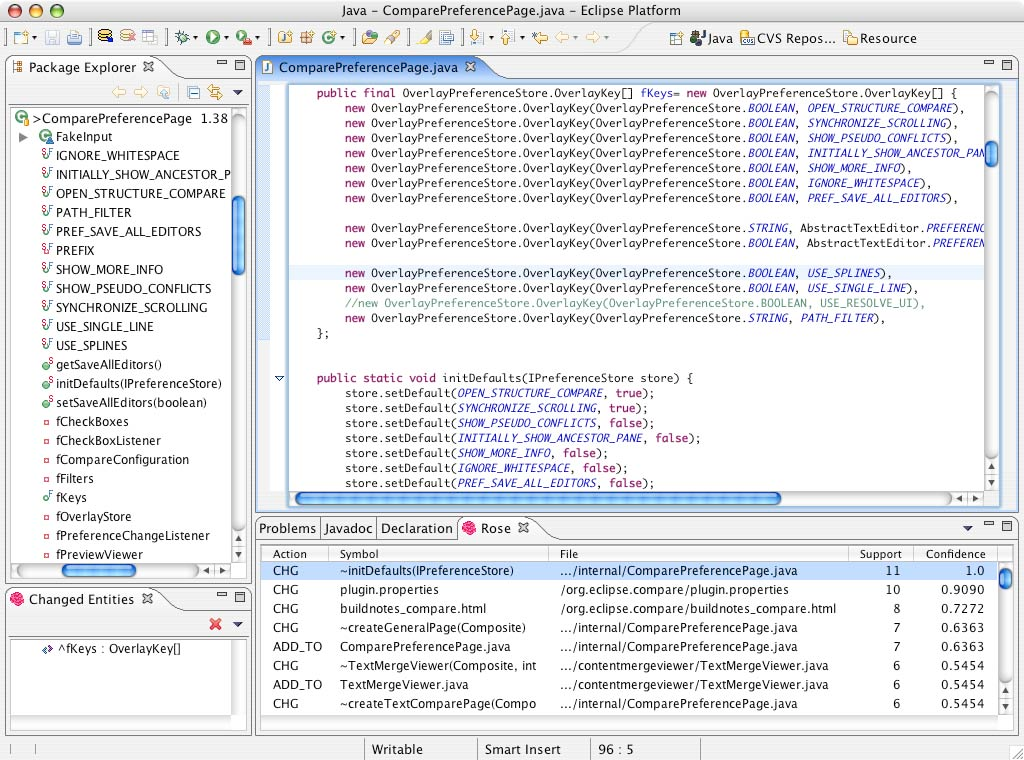
\includegraphics[scale=0.4]{rose}
\centering
\caption{eRose plugin}\label{rose}
\label{fig:rose}
\end{figure}

\subsection{Strathcona}
Another example is the Strathcona system \cite{strathcona} which extracts data about the structure of a code fragment in order to search a PostgreSQL database and use heuristics to rank the results. It shows a structural overview, as well as highlights based on the difference from the user's code. This system is particularly useful for frameworks that have been poorly documented.

\begin{figure}[H]
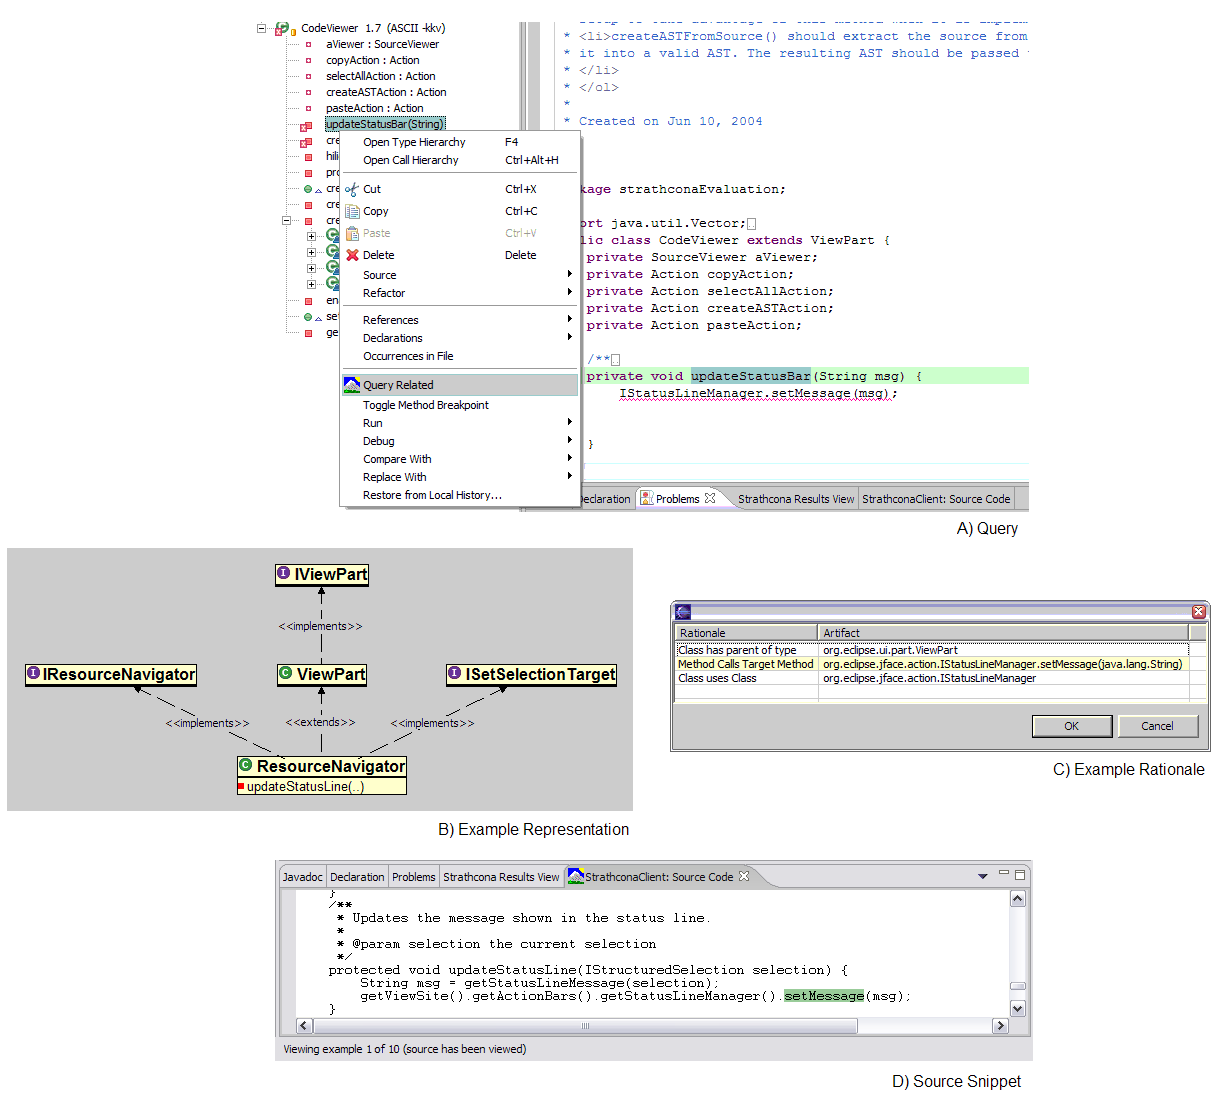
\includegraphics[scale=0.26]{strathcona}
\centering
\caption{Strathcona plugin}\label{strathcona}
\label{fig:strathcona}
\end{figure}

\newpage
\subsection{Suade}
Suade \cite{suade} is also an Eclipse plugin which is specialised in automatically presenting suggestions by retrieving related elements (fields, methods). By design, it contains a dependency graph of the elements that can be interactively and iteratively updated by the developer.

\begin{figure}[H]
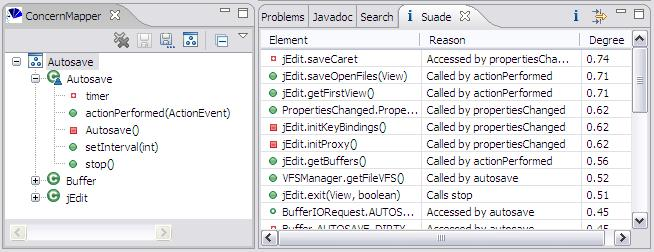
\includegraphics[scale=0.9]{suade}
\centering
\caption{Suade plugin}\label{suade}
\label{fig:suade}
\end{figure}

\subsection{CodeBroker}
CodeBroker \cite{codebroker} uses as input the comments written by developers to assist them. A recommendation is produced every time a comment is written by analyzing the text and doing type-signature matching. The system also manages user-specific lists.

\begin{figure}[H]
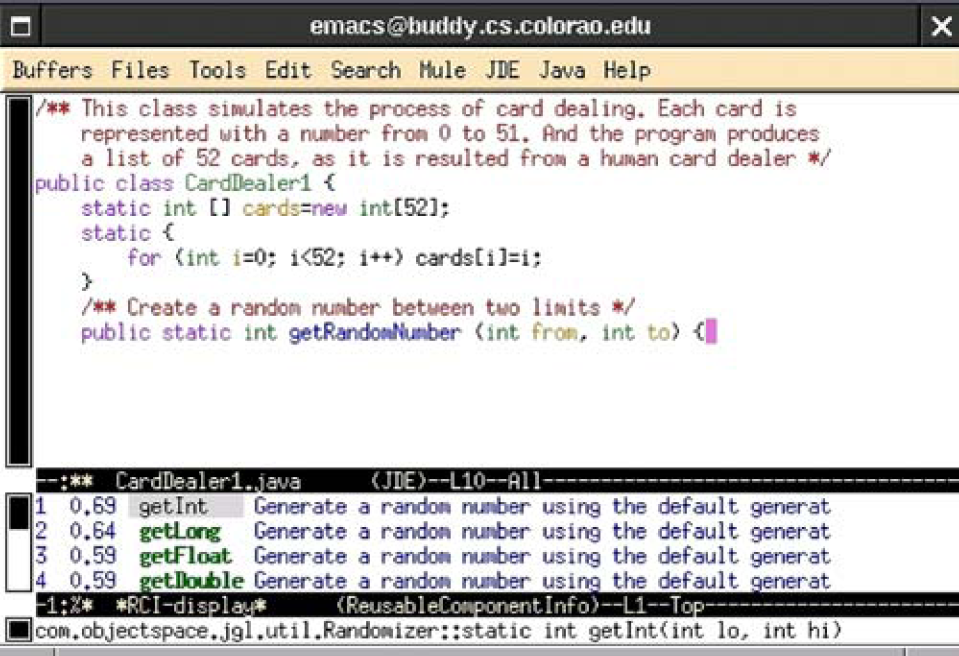
\includegraphics[scale=0.4]{code-broker}
\centering
\caption{CodeBroker plugin}\label{code-broker}
\label{fig:code-broker}
\end{figure}

\subsection{Dhruv}
Dhruv \cite{dhruv} is a system that recommends people and artifacts based on bug reports. It extracts data from the open source community (different types of users and content and their interactions) to create a Semantic Web, which later is used to match that to the bug report's information.

\begin{figure}[H]
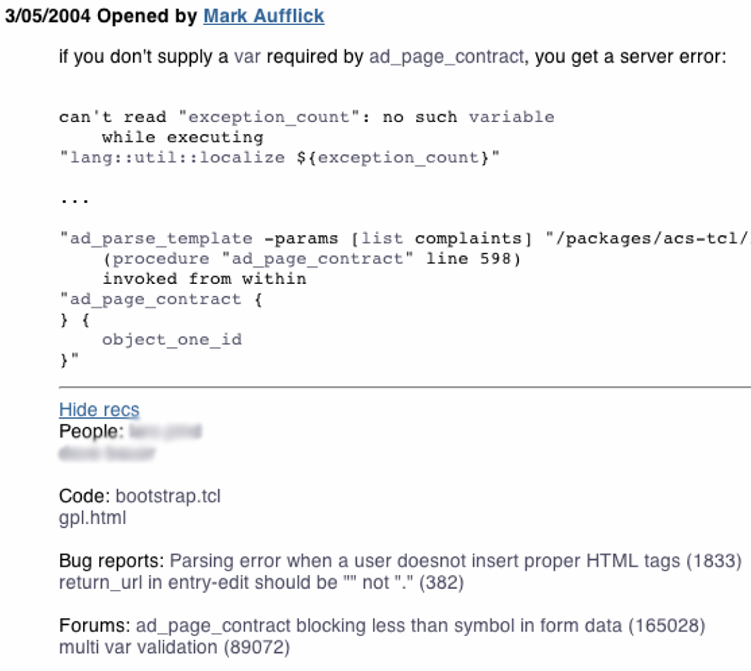
\includegraphics[scale=0.45]{dhruv}
\centering
\caption{Dhruv plugin}\label{dhruv}
\label{fig:dhruv}
\end{figure}

\subsection{Expertise Browser}
Expertise Browser \cite{expertisebrowser} recommends people for a particular piece of code by considering the people who have modified the content in the past. However, an assumption is made that whoever made changes beforehand is an expert.

\begin{figure}[H]
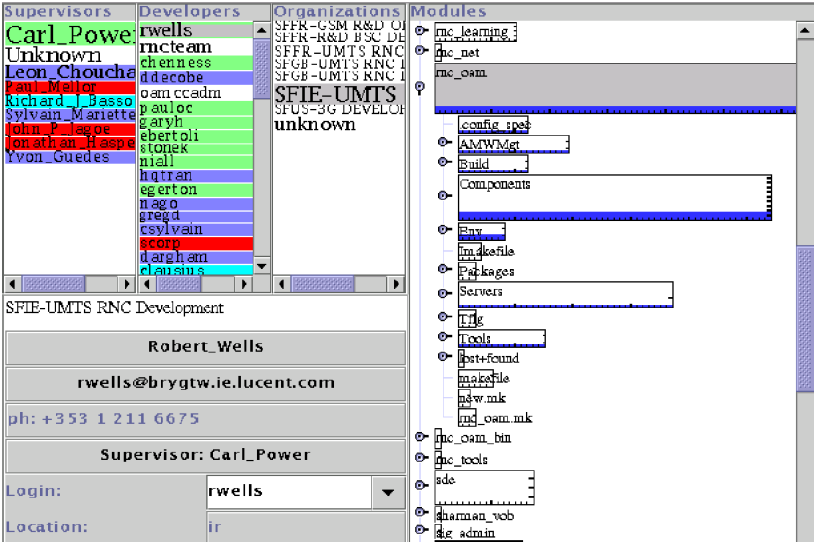
\includegraphics[scale=0.4]{expertise}
\centering
\caption{Expertise Browser recommender}\label{expertise}
\label{fig:expertise}
\end{figure}

\subsection{ParseWeb}
ParseWeb \cite{parseweb} is useful in situations when the developer needs an object to perform methods on, but cannot recall how to get the object. The tool crawls the web based on the user's input (object types) to search for recommendations.

\begin{figure}[H]
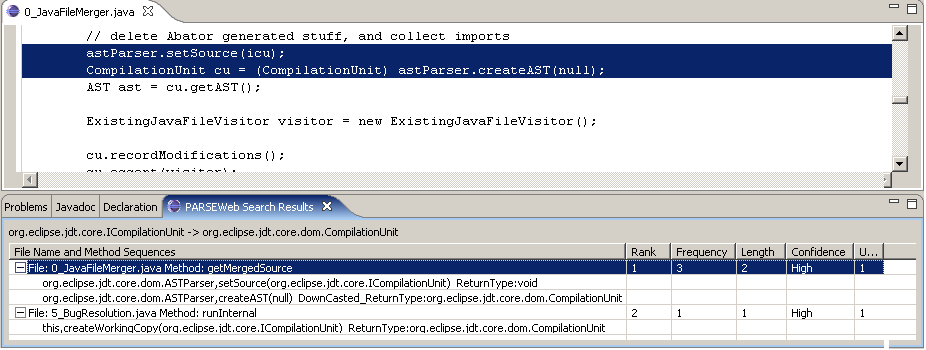
\includegraphics[scale=0.5]{parseweb}
\centering
\caption{ParseWeb recommender}\label{parseweb}
\label{fig:parseweb}
\end{figure}

\subsection{Autocomplete with Stack Overflow}
Autocomplete with Stack Overflow \cite{autocomplete-so} provides code snippets from Stack Overflow answers with more than 50 upvotes for the JavaScript language.

\begin{figure}[H]
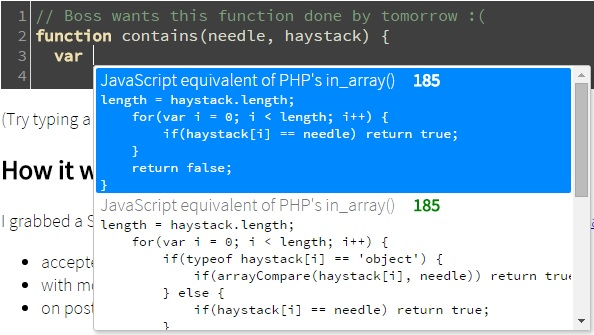
\includegraphics[scale=0.8]{autocomplete}
\centering
\caption{Autocomplete with Stack Overflow}\label{autocomplete}
\label{fig:autocomplete}
\end{figure}

\newpage
\subsection{Evaluation of Similar Ideas}
As it was already stated most systems and tools described above have something in common - they do recommendation by going through several stages - input handling, intermediate analyzing of some sort, and visualisation technique. However, they also have a unique approach that is very specific and focuses on certain aspects - for example, the Autocomplete with Stack Overflow approach gives only snippets with more than 50 upvotes. Existing code recommendation by the IDE's do not give example code, but rather offer small suggestions to the code. Source Code Clippy is special because it offers helpful features to assist the developer and mainly because it features different ways of searching for excerpts by focusing on getting data from Stack Overflow - one of the biggest sources of code snippets and a part of the Stack Exchange network of websites. Stack Overflow has more than 5 million users, which write about 3 questions and 4-5 answers each minute (based on average statistics ). So far the website has more than 11 million questions and 18 million answers in total.

\section{Description of Tomasz's Prototype}
The Source Code Clippy plugin is a continuation of an already build unevaluated prototype for Sublime which Tomasz Sadowski developed.

\noindent
The prototype initially used python scripts to make queries to the Stack Overflow API and save the data returned. Scripts have been created to visualize this data in graphs - for example, to compare the popularity of the most used tags. However, because limited number of request can be made, the data was gathered from a dump provided by Stack Overflow in the form of XML files. The posts, tags, users, votes and comments data was parsed and imported to a custom created PostgreSQL database. Queries for querying the database with some simple queries such as get answers for a specific question id, as well as queries that process the tags were used. Finally, the Terrier information retrieval platform was explored as a possibility for faster search.

\noindent
In practice, a developer could be working on a script to process text files and has started on the task of opening files. The recommender tool searches for relevant code snippets and presents them for auto insertion into the editor. 

\chapter{Requirements}

\section{Requirements Elicitation and Gathering}
Requirements were gathered and discussed during informal weekly customer meetings - new requirements were added throughout the iterations. The project was hosted on GitHub \cite{github} and the available issue tracker \cite{github-issues} was used to list and track the progress of each requirement along with the tasks involved that needed to be completed.

\section{Functional Requirements}
The functional requirements define what the system is expected to do. These requirements  were prioritised based on the MoSCoW approach \cite{moscow}. The final list of all collected requirements is split into tables based on their priority and are also presented below.

\subsection{Must Have}
Must have requirements are fundamental and crucial to the success of the project. Table ~\ref{table:mustTable} shows the details of the must-have requirements. In short, the requirements are responsible for the distinct types of searching and their settings settings, as well as handling the different user input.

\begingroup
\renewcommand\arraystretch{1.5}
\begin{longtable}{p{0.5cm}p{4cm}p{9cm}p{2cm}}
\caption{Must Have Requirements}\\
\hline
FR & Requirement & Description & Date \\
\hline
1 & Searching with local index & Based on some input, the user must be able to search using an index on the local file system, as well as create a new index/update existing one. & 5 Nov 2015\\
2 & Searching with Stack Exchange API & The user must be allowed to make requests to the Stack Exchange API based on a query and see the results returned & 30 Nov 2015\\
3 & Searching using a Web Service & The user must have the option to choose to search using a web service - a preindexed collection of Stack Overflow question and answer posts & 13 Jan 2016\\
4 & Searching with Google for the Stack Overflow domain & The user must be given the option to choose to search the text in the query pane with Google & 18 Dec 2015\\
5 & Configuration panel & The user must be provided with the functionality to change the settings of the plugin in order to configure and customize it to their needs - changing the local index used, the web service URI, etc & 30 Nov 2015\\
6 & Handling selection input & The user's mouse selection should be automatically & 16 Nov 2015\\
7 & Last statement typed query input & The user's key input should be captured and update the query input pane & 5 Nov 2015\\

\hline
\label{table:mustTable}
\end{longtable}
\endgroup

\subsection{Should Have}
The should have requirements are considered as important but not critical to the system. Table ~\ref{table:shouldTable} represents all the 'should have' requirements along with their description. To summarize, the list contains the additional features that make interaction much easier - like the feedback tab, sorting, filtering, importing code easily, etc.

\begin{table}[H]
\caption{Should Have Requirements}
\centering
\def\arraystretch{1.5}
\begin{tabular}{p{0.5cm}p{4cm}p{9cm}p{2cm}}
\hline
FR & Requirement & Description & Date \\
\hline
8 & Insertion of code by double clicking a post & The user should be able to automatically import code into the editor by double clicking & 5 Nov 2015\\
9 & Filters of results & The user should be able to filter the results from search by the minimum number of upvotes & 30 Nov 2015\\
10 & Feedback tab & The goal is to improve the system and therefore the user should be able to submit feedback & 27 Jan 2016\\
11 & Display post useful meta data information and offer customization to the post & Posts should contain their type (question or answer), their score (if applicable) and a hyperlink leading to their source. There should be options to customize the post - let the user choose the text colour used, etc. & 20 Jan 2016\\
12 & Custom input pane listener & The user should be able to make search request on 'Enter' and new lines with the 'Shift' key when the focus is on the query pane & 30 Nov 2015\\
13 & Additional search request & The plugin should offer an additional search request to be made on the same query to allow more posts to be fetched and displayed & 30 Nov 2015\\
14 & Sorting results & The user should be able to sort results by relevance or by score & 20 Jan 2016\\
\hline
\end{tabular}
\label{table:shouldTable}
\end{table}

\subsection{Could Have}
Could have requirements are optional features the system could benefit from. Due to time constraints, FR21 was not implemented, but is considered for possible future work. Table ~\ref{table:couldTable}  lists the 'could have' requirements, as well as their descriptions. The list presents the nice to have features such as highlights on code, information tab, changing the number of posts, etc.

\begin{table}[H]
\caption{Could Have Requirements}
\centering
\def\arraystretch{1.5}
\begin{tabular}{p{0.5cm}p{4cm}p{9cm}p{2cm}}
\hline
FR & Requirement & Description & Date \\
\hline
15 & Number of calls to Stack Exchange API & The plugin could display the remaining calls that can be made to the API & 27 Jan 2016\\
16 & Highlighting code & Highlighting the text in HTML code tags to distinguish between code and text of a post & 5 Nov 2015\\
17 & Write a question & Functionality to enable the user to write a question on Stack Overflow & 20 Jan 2016\\
18 & Information tab & A tab for showing information to the user that they might need to know & 27 Jan 2016\\
19 & Default number of posts and max number of posts & Feature which gives the user the ability to change how many post they see after a search (on 'Enter'), and a secondary search (using the scroll) & 20 Jan 2016\\
20 & Saved settings & The options the user selects and changes could be saved automatically and loaded when the plugin starts & 20 Jan 2016\\
21 & Code Intelligent Search & The variable names and other terms in the query that are less relevant could have less weight attributed to them so that the results are more refined. The use of tags that allow the user to filter could be also a potential improvement. & 30 Nov 2015\\
\hline
\end{tabular}
\label{table:couldTable}
\end{table}

\newpage
\section{Non-Functional Requirements}
Non-functional requirements represent the qualities the system is required to meet. Table ~\ref{table:nonFuncTable}  lists and describes the non-functional requirements for the plugin that were decided at the start of the project.
\begin{table}[H]
\caption{Non-Functional Requirements}
\centering
\def\arraystretch{1.5}
\begin{tabular}{p{2cm}p{4cm}p{9cm}}
\hline
NFR & Requirement & Description \\
\hline
1 & High performance & The user should not have to wait more than a few seconds when executing a query for just a few results. Performance should not sharply and unbearably decrease when the user wishes to get more results back \\
2 & High usability & Users should not get confused and feel the plugin as something they are familiar with - the user interface should be intuitive. The plugin should have good responsiveness, but also provide helpful features e.g. automating the process if possible and reasonable to do so \\
3 & Extensible with good documentation& The system should allow for easy future extensions. Well-documented code allows for easy extension of the plugin\\
\hline
\end{tabular}
\label{table:nonFuncTable}
\end{table}

\section{Use Cases}
A list summarizing the different use cases follows.

\begin{itemize}
\item The user can update the query pane in various ways - directly, by mouse selection, or key input.
\item The user can choose to search from a number of sources.
\item The user can sort and filter results.

\item The user can execute a query
\begin{itemize}
\item The user can make another request that will provide more results.
\item The user can import code by double clicking on code from posts
\item The user can see meta data about each result/post
\end{itemize}

\item The user is allowed to view the past search history. 
\item The user can change the settings and any changes made are saved so they can be loaded on startup.
\item The user can see information about the plugin that will serve as a guide
\item The user can provide feedback and contact the developer if they need to
\end{itemize}

\chapter{Design and Implementation}

This chapter includes an explanation of the developer's workflow, an overview of the iterations and the decisions made for the design and implementation of the initial and final designs.

\section{Developer's Workflow}
Based on the use cases outlined, the typical developer workflow consists of typing a query by using the easiest way (might be mouse selection or automatically captured key input); searching for the result by changing the query in an iterative manner and the search method used appropriately until they find the result needed. Using the useful options provided (e.g. extended search, double click to import, etc) can speed up the process of completing the task being worked on.

\noindent
In the UML Activity diagram \ref{fig:activity-diagram} an example workflow that uses a combination of use cases (which are coloured in orange) is demonstrated:
\begin{enumerate}
\item The user opens the plugin
\item The user has the option to type something in the query pane
\item The user executes that query

\begin{enumerate}
\item Results are returned. The user is allowed to do the following:
\begin{itemize}
\item An extra search for that query
\item Double click on a code snippet to import it in case it is permitted (web service search was used)
\end{itemize}
\item Results are not returned - an error notification is shown.  
\end{enumerate}

\item The user is allowed to change the search strategy used
\item The user is allowed to go back to (2)
\item Finally, the user clicks on the 'Ask a question' because they have made sure they have not found an appropriate code snippet to the question or any explanation about the task. 
\item The user is allowed to go back to (2).
\item The process of interaction with the plugin ends intentionally when the user closes IntelliJ.
\end{enumerate}

\begin{figure}[H]
\includegraphics[scale=0.5]{activity-diagram}
\centering
\caption{UML Activity diagram}\label{activity-diagram}
\label{fig:activity-diagram}
\end{figure}

\section{Iterations Overview}
Consecutive iterations of developing the plugin consisted of several stages:

\subsection{Familiarisation and Preparation}
The first iterations consisted of familiarizing with how to develop a plugin for IntelliJ, how to do indexing and searching programmatically, and extracting data from the given PostgreSQL database. The database consists of a single table with the identifiers of posts and their data - such as parent id (for an answer that will be question id), score and others.

\subsection{Implementation of the Plugin}
This stage consisted of building an initial version of the plugin that uses a local index, as well as Stack Exchange API search. Basic functionality such as code highlighting were also implemented.

\subsection{Expanding and Improving the Plugin}
The next iterations until the end of the project required developing a web service, automating existing features (input on selection and typing, copying code into editor, etc) and implementing new features such as adding configuration settings, search history, additional search options, feedback and information tabs.

\subsection{Evaluation}
Tests were implemented to test the functionality of the system. Various code metrics were used to determine the implementation quality of the plugin. User evaluation was carried out to better understand how useful the implemented features of the plugin are to developers in practice. 

\newpage
\section{Architecture}
Consecutive iterations of implementation caused the plugin's architecture to change. The figures \ref{fig:architecture-initial} and \ref{fig:architecture} use special colouring to differentiate different components - the logical parts of the system are coloured in red. The data sources can be identified by their green colour. The boxes in blue represent outgoing links.

\subsection{Initial Architecture}

\begin{figure}[H]
\includegraphics[scale=0.4]{scc-architecture-initial}
\centering
\caption{Architecture diagram}\label{scc-architecture-initial}
\label{fig:architecture-initial}
\end{figure}

The project was initially required to use a local index on the PostgreSQL database given by Tomasz. A decision was made to export only the relevant data - Java questions and answers - and perform indexing on those posts. 
\\
\\
Implementation wise, the process of extracting files from the initially provided database consists of the following steps:
\begin{enumerate}
  \item Writing a query for retrieving questions and another one for answers, both of which add extra empty column for record separation.

\begin{lstlisting}
# Extracts questions
SELECT Posts.*, '' AS LineEnding
FROM Posts
WHERE Posts.tags LIKE '%<java>%'
\end{lstlisting}

\begin{lstlisting}
# Extracts answers
SELECT P1.*, P2.*, '' AS LineEnding
FROM Posts AS P1 JOIN Posts AS P2 ON P1.id = P2.parentid
WHERE P1.tags LIKE '%<java>%'
\end{lstlisting}

\item Exporting the results to a CSV file with a unique separator
\item Using a custom written CSV splitter to create the files used for indexing purposes
\end{enumerate}

\noindent
The plugin was also needed to retrieve code snippets by using Stack Exchange's API. Since the project is about retrieving code snippets, it was decided from the documentation that the plugin would use the 'excerpts' method provided. The response from all API methods is in the form of JSON objects.

\subsection{Final Architecture}

\begin{figure}[H]
\includegraphics[scale=0.5]{scc-architecture}
\centering
\caption{Architecture diagram}
\label{fig:architecture}
\end{figure}

During the different iterations, it was clear that a local index was not a good enough option as it required every plugin user to have the files stored on disk. Therefore, a web service was created to replace the local index and replace the need for storage on each machine/client. However, it was seen that a local index could still be beneficial if the user wished to index a collection of their own documents. Thus, it was decided that the local index remained as a feature that provides a different and unique type of search.

\noindent
The extraction of data from the database and extracting files from the CSV exported files required steps, which did not need to be made. Instead, it was discovered that indexing on the database could be done directly - this is a more straightforward way of indexing and minimizes the time taken to do the steps described which take a lot of time.

\noindent
Searching with Google was added as an option to test how useful that would be to the user when related code snippets are involved.

\noindent
To sum up, the user can use the IntelliJ Scclippy plugin to retrieve excerpts data from a number of data sources:

\begin{itemize}
\item by using a local index on the user's file system that can be changed.
\item by sending requests to the Web Service which in return will return a JSON response
\item by using the Stack Exchange API to make the request.
\item by clicking on a button that will open a browser window and search the query using Google for the domain of Stack Overflow. 
\end{itemize}

\noindent
The system also has a hyperlink to each post returned, as well as to an online survey that the user can follow, fill and submit online. 

\noindent
The client automatically saves its settings to a file relative to the plugin's installation in order to load them when a new IntelliJ client is started and the plugin was launched. Each instance of IntelliJ contains a separate instance of the Scclippy plugin.

\section{Design}

\subsection{Package Diagram}
The code written for the client was organized into two layers - business and presentation. The UML package diagram \ref{fig:scc-package-diagram} shows the design of the plugin by illustrating the different packages responsible for those layers as well as their composing packages. The business logic is handled in the package named 'plugin' and the presentation logic in the one named 'uicomponents'. All unnamed dependencies are of type "uses" - for example, the 'uicomponents.search' package uses the 'plugin.lucene' package because it needs the File class that was defined there - an import is needed so that the posts returned by searching are meaningful and can be displayed. The 'uicomponents.main' creates all tabs when the plugin is started. It also uses the 'uicomponents.search' package to update the input pane with the editor mouse selection string.

\begin{figure}[H]
\includegraphics[scale=0.5]{scc-package-diagram}
\centering
\caption{UML Package diagram}
\label{fig:scc-package-diagram}
\end{figure}

\newpage
\subsection{Class Diagrams}

Class diagrams for two of the vital packages for the system have been examined.

\begin{figure}[H]
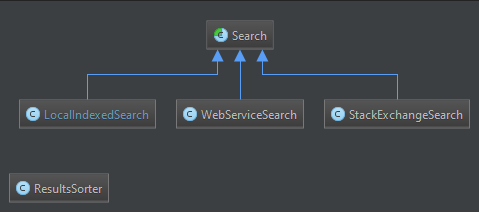
\includegraphics[scale=0.8]{search-classdiagram}
\centering
\caption{Class diagram for package 'plugin.search'}
\label{fig:search-classdiagram}
\end{figure}

\noindent
Diagram ~\ref{fig:search-classdiagram} shows the structure of classes for the 'plugin.search' package and how the different search methods are implemented as separate classes that extend the 'Search' abstract class. New search options can be added easily. The ResultSorter is used for sorting results.
\\
\\
\begin{figure}[H]
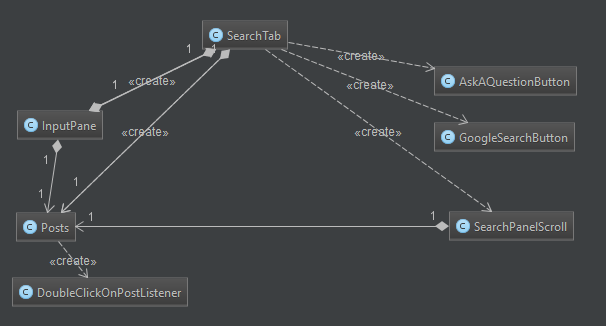
\includegraphics[scale=0.8]{searchtab-classdiagram}
\centering
\caption{Class diagram for package 'uicomponents.search'}
\label{fig:searchtab-classdiagram}
\end{figure}

\noindent
The class diagram ~\ref{fig:searchtab-classdiagram} represents the structure of classes inside the 'uicomponents.search' package. Each class represents a user interface component. The SearchTab contains a panel  in which every other directly connected component is placed in the tab. Posts create their own mouse listeners. In order to perform search the InputPane and SearchPanelScroll must know about the object responsible for that purpose, as well as be able to modify the content of the posts by calling the appropriate methods. In addition, the InputPane is also given the history tab as a parameter to update the search history. This structure of the code (with tabs, panels and components) is also valid for the other user interface packages and allows easy expansion of the plugin with new functionality.

\newpage
\section{Libraries Used}

The table below shows the different libraries, their description and the version used for the implementation of the client and the server parts of the project.

\begin{table}[H]
\caption{Libraries used}
\centering
\def\arraystretch{1.5}
\begin{tabular}{p{4cm}p{9cm}p{2cm}}
\hline
Library & Description & Version \\
\hline
junit & Used for unit testing purposes & latest \\
org.json & Used by the client to read the response from the web service or Stack Exchange API & 20140107 \\
com.googlecode.json-simple & Used by the web service to create a reply & 1.1 \\
org.apache.lucene & Used for information retrieval indexing and searching. Includes lucene-core, lucene-analyzers-common, lucene-queryparser artifacts& 5.3.1 \\
com.sun.jersey & For building the RESTful web service & 1.8 \\
net.sf.trove4j & Provides optimized primitive collections for Java & 3.0.3 \\
org.postgresql & For accessing the PostreSQL database & 9.4.1208.jre7 \\
\hline
\end{tabular}
\label{table:librariesUsed}
\end{table}


\section{User Interface}
The user interface was also changed frequently in order to keep up with the dynamic requirements and new features each iteration, but also due to ideas about improvements to make the look and feel of the plugin better. The differences of the basic and final design are shown below in terms of architecture and user interface.

\subsection{Sketches}

\begin{figure}[H]
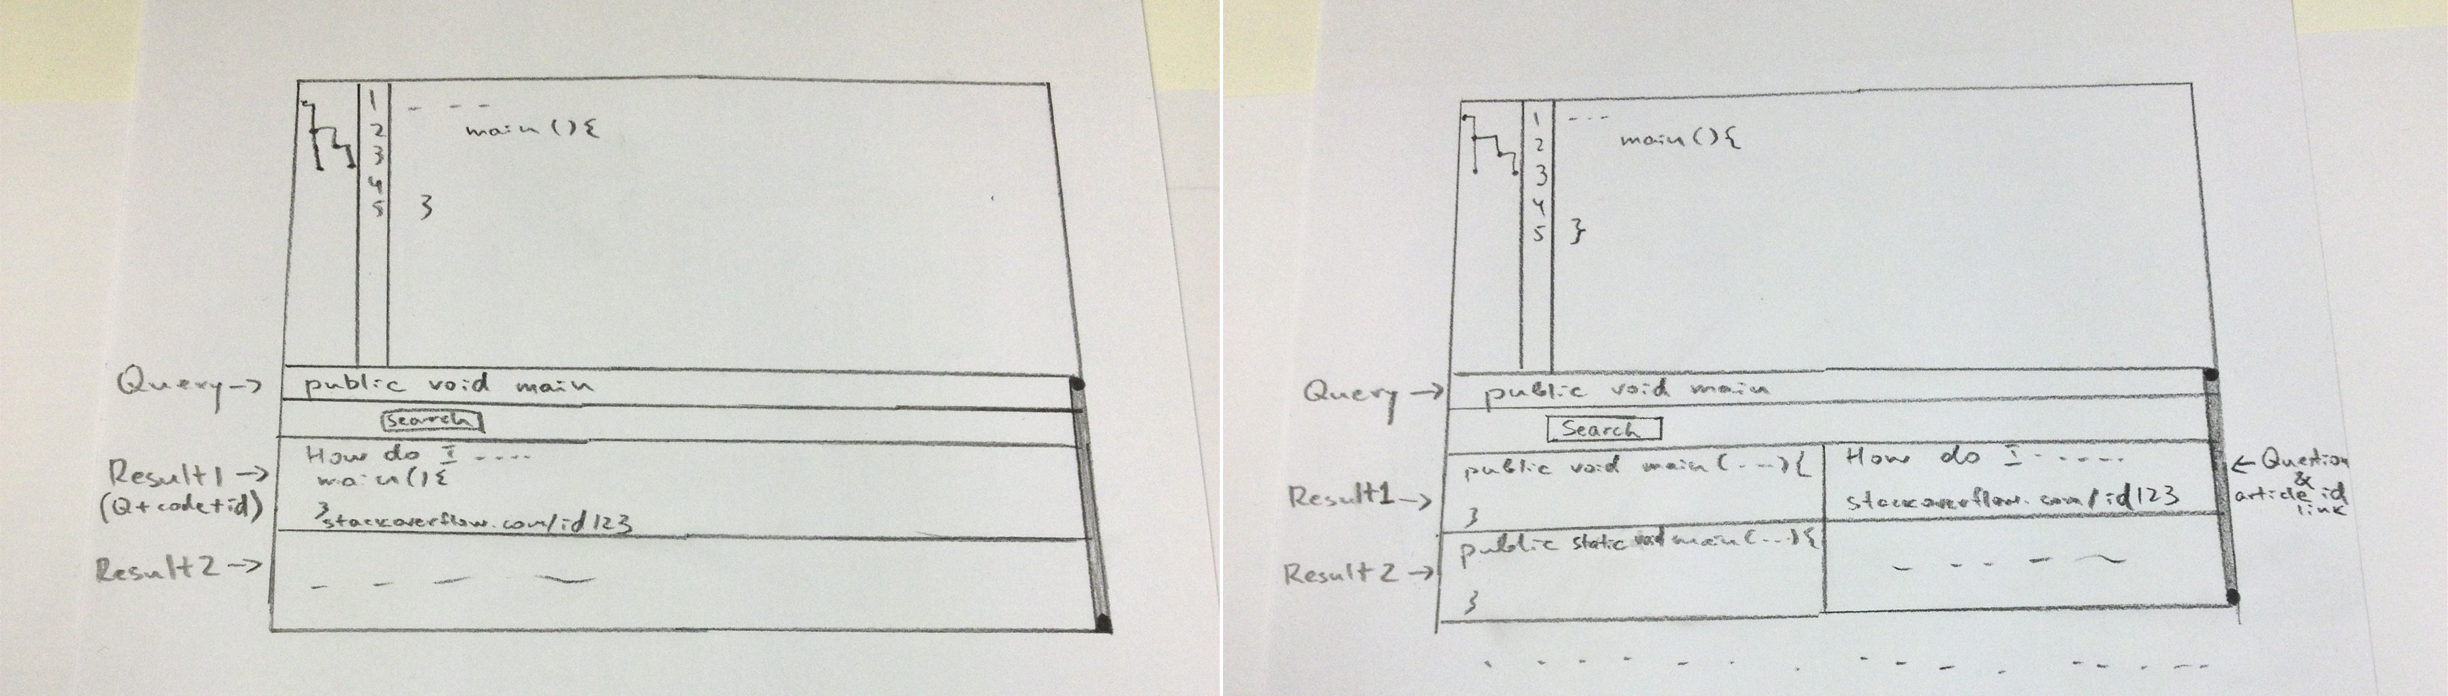
\includegraphics[scale=0.2]{sketches}
\centering
\caption{Sketches of the proposed User Interface designs}\label{sketches}
\label{fig:sketches}
\end{figure}

In the beginning of this project, two sketches of how the plugin would look like were proposed. Both of them share some of the design choices made - the query pane to be located at the top with a button for searching (using Stack Overflow) immediately after. The designs differ mainly in how posts are displayed - the first keeps the whole posts one after another, while the latter splits the code from the text and the link to the post. The first design was chosen to be implemented as it is more simple and it might be disturbing for the user to look left and right for the information needed, especially if multiple code snippets, small or long in size, are involved. The latter design also could be problematic if the user has opened another tool window beside the one used for Scclippy - then the user is required to use a horizontal scroll to see the details of the post which is inconvenient. This is why whenever a new feature was added to the plugin, the position of that element was considered to be better if it were placed on the left side of the panel so that the user should not need to scroll to the right.

\subsection{Initial Design}
\begin{figure}[H]
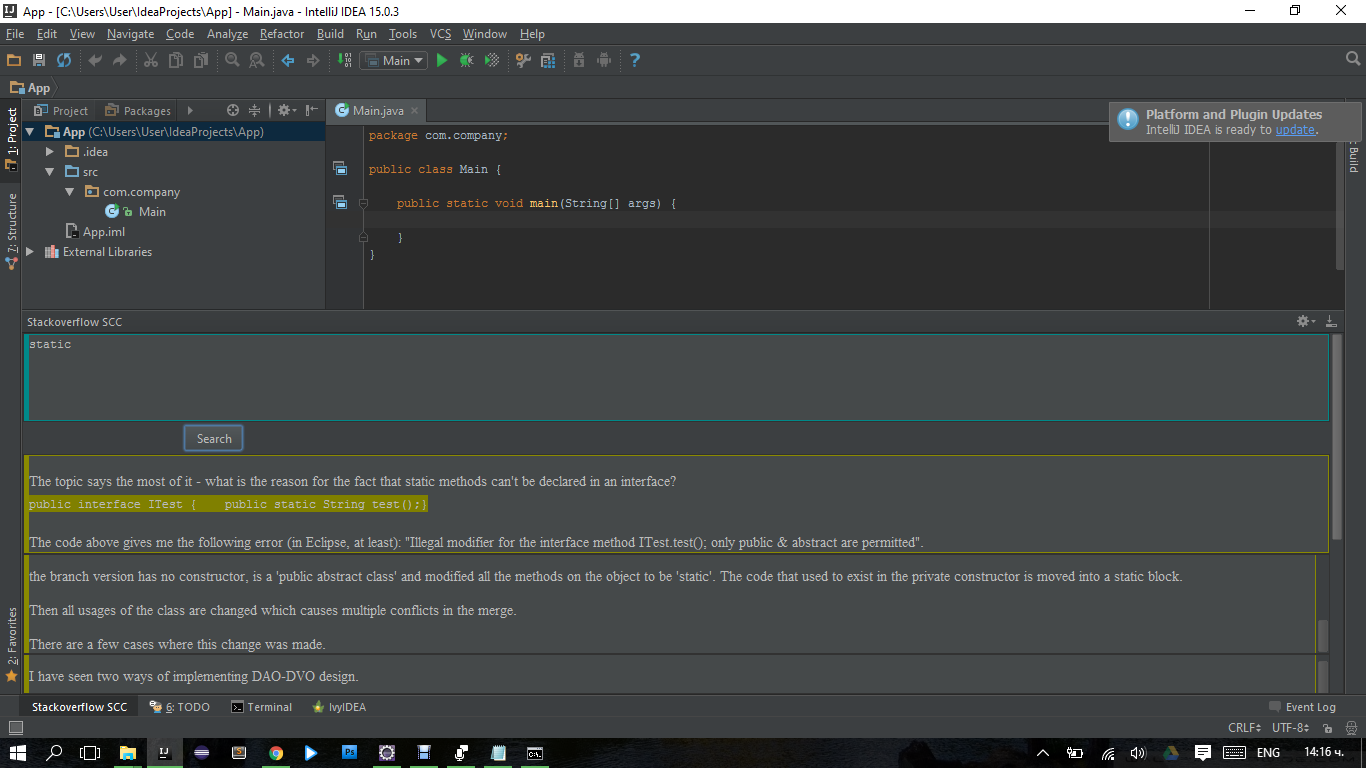
\includegraphics[scale=0.5]{ui-old}
\centering
\caption{Initial User Interface design}\label{ui-old}
\label{fig:ui-old}
\end{figure}

As a result, you can see that the first sketch was implemented successfully in the first iterations of the project. The code is highlighted on purpose so that the user is more aware of the presence of the code snippets in the post and their positions respectively.

\subsection{Final Design}
The final user interface design has introduced several tabs to handle all the different features of the plugin. The next section discusses the design along with the features of the plugin.

\section{Final Design - Features and Decisions}
This section will discuss the finalized features of the system and the different choices made throughout all iterations by comparing them using their pros and cons. The decisions taken aim to make the system meet the functional and non functional requirements in the best way possible. 

\noindent
The plugin has its own closable window (ToolWindow) in IntelliJ that features five tabs. The function of each tab and its components is explained below.

\subsection{General Design Decisions}

\subsubsection{Programming language and IDE choices}
Java was the programming language chosen and IntelliJ was picked due to their popularity - Java is frequently used among developers, while IntelliJ is also widely used and in addition offers very useful features to programmers - which were used even when developing the plugin.

\subsubsection{Java Swing vs Java FX}
The plugin's user interface was chosen to be implemented with the Java Swing toolkit rather than Java FX mainly because of familiarity reasons.

\subsubsection{Indexing and Full-Text Search}
Indexing was regarded as more suitable than Full-Text search to do the task of retrieving code snippets. The main reason is that indexing platforms are more efficient and flexible - they offer more customization and retrieval is done much faster.

\subsubsection{Lucene and Other Retrieval Platforms}
The choice of an open source information retrieval platform came down mainly from easiness of implementation. Terrier did not have a proper straightforward tutorial showing a programmatic way of calling the API. Apache Lucene Core (https://lucene.apache.org/core/) was used for indexing and retrieval of files. Since there were no problems, and the platform was sufficiently good for the plugin, other options were not considered. Each retrieval platform has its own implementation and principles, however, it should be pointed out that the decision made does not mean a less capable system was used. Apache Solr which uses Lucene could be considered as an alternative and an improvement in the future as it offers more features.

\subsubsection{Lucene Settings}
\begin{itemize}

\item Stopwords were removed as most code is filtered out due to insufficient length and that is not what the plugin needs - for example, keywords are often short and should not be filtered.

\item No stemming is applied since retrieval is fast and there is no need to make the underlying dictionary small and sacrifice details. In terms of precision, the effectiveness of stemming were not compared to those without stemming. 

\item Pruning - neither document-based, nor term-based pruning was used for the same reason stemming was not used.

\item Special characters are escaped when querying to enable braces and other useful symbols 

\item Default scoring settings were used \cite{lucene-scoring}:

\begin{itemize}
\item Frequent terms in a document increase the documents score
\item Popular terms have lower score
\item More terms that match the query means higher score
\item Short documents are preferred over long documents 
\end{itemize}

\end{itemize}

\subsubsection{IntelliJ Notifications} 
IntelliJ notifications are used to inform the user with the outcome of their actions. Examples include "Check connection to server. ..." which is displayed when the user is not connected to the Internet or other connection problems have occurred.


\subsection{Search Tab}

\begin{figure}[H]
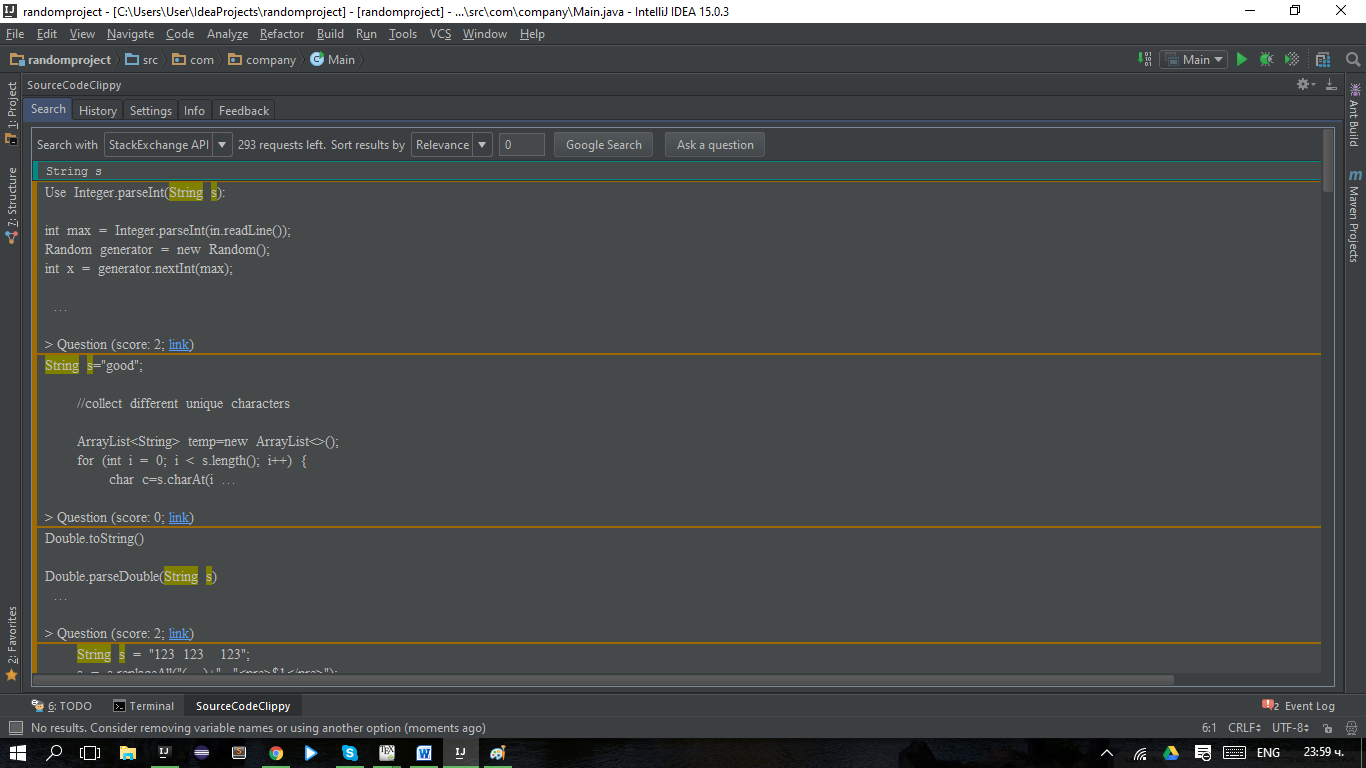
\includegraphics[scale=0.5]{tab-search}
\centering
\caption{Search tab, Darcula IntelliJ theme}
\label{fig:search-tab}
\end{figure}

\subsubsection{Search Methods}
The search tab contains four different types of search for excerpts - one for Google search with the domain of Stack Overflow (clickable by a button) and the rest three grouped together are selectable by a combo box. The latter were eventually grouped together because they changed the posts displayed inside IntelliJ, while the Google button's functionality is different.

\noindent
The reason for having so many options is that searching for code snippets with one method e.g. Stack Exchange API was not enough as it had its limitations and other ways that can provide additional useful results existed. Therefore, the system offers a number of techniques for searching excerpts that have been outlined below:

\begin{itemize}

\item \textbf{Local Index} - offers the user to freely create/update an index on a chosen data set. The major benefit of this approach is that the user can use it while being offline. The downside is that it requires documents, which the user might need, but does not have on their machine - if the user requires more information, about a topic, they may likely not have it.  

\item \textbf{Web Service} - has an already indexed collection of Stack Overflow posts for the Java programming language.  The benefit of the web service is that it covers a large dataset - about 2 million documents. In addition, it offers unlimited requests. The negative side is that it is not kept up to date like the Stack Exchange API. 
\\
\\
This method required creating a custom server that provides a RESTful Web Service that on requests performs search using Apache Lucene and returns only the number of documents specified (default is 5) that contain the id, body and score for each post. 
Initially, the server used Lucene to index the extracted files, however a decision was made to make the server use an index on the given PostgreSQL. This approach minimizes the steps needed to index the required posts.
\\
\\
The web service was deployed to an application server (rote.dcs.gla.ac.uk:9999). The major downside is that the it is only available to certain users which need to tunnel to the University's network and login with their credentials in order to have access. The server could have been deployed in the cloud to overcome this problem. However, different providers provide different solutions. For example, some of them do not offer PostgreSQL database support. Deploying the system itself has its own challenges - ideally, it should be done with minimal change of code. The plugin does not feature integration with cloud services. 

\item \textbf{Stack Exchange excerpts API} \cite{stackexchange-excerpts} - uses the excerpts method provided by the v2.2 API to retrieve up to date Stack Overflow snippets. Each user has a limited number of requests, equal to 300 daily (by default). The number of calls left are displayed in a pane right to the combo box and is automatically hidden for other options. Another downside is that this approach depends on variable names e.g. in the worst case if the user chooses to search for a something with a very specific variable name (e.g. 'String \textit{hsaudhqwudhyqgwd} = "";') then most likely they will not get any results back.

\item \textbf{Google Search} - opens a browser tab that searches using the index created by Google on the Stack Overflow's domain. This is a generally good option since it is not so variable independent as the previous type of search.

\end{itemize} 

\noindent
All of the above methods use an index to process requests quickly and thus make the plugin more usable. Since they use a different ranking mechanism, the result they return when queried will be different from the others.

\subsubsection{Query Input Pane}
The input field can be used by directly typing into it. Search is performed when 'Enter' is typed in the query pane which the user can use to write a query. The 'Shift + Enter' key combination was used as a replacement for the 'new line' command.

\textbf{Executing a query} options include:
\begin{itemize}
\item Standard way - using a simple button
\item Automatic search listener which listens for any activity (typing, deleting or pasting text) which saves time – one less click per query - and is more intuitive.
\item Search on 'Enter' key pressed. This decision, to remove the button and introduce this functionality, was made to speed up the process of user interaction with the system as it is faster than using a button. Automatic search seems the best in terms of speed of execution, but in practice, it was changed in one of the iterations so as to avoid too many requests as there is a limit on the requests that can be made to Stack Overflow, and to avoid sending too many requests to the web service as they will not be handled at a sufficient pace.
\end{itemize}

\textbf{Code insertion from editor to query pane} could be done in multiple ways:

\begin{itemize}
\item Standard copy paste - available by default.
\item When selecting text the user could right click and select an option to allow him to set the text of the query (search begins automatically). This was used in the first iterations, but changed later.   
\item Instant copy paste on selection. Compared to the previous approach, the user usually wishes to change the query quickly and most of the times they update the query pane when they are finished looking at the information about the current search. Thus, this was chosen to be implemented for the final design of the plugin due to better usability and efficiency.
\end{itemize}

\noindent
When \textbf{typing} the input field is set to contain the text being typed. The text that is captured is triggered on special characters and the text of the last command range is restricted to the last seen semi colon or brace. This way only the relevant text being typed is considered and the approach also prevents ranges of text starting from import statements. The method does not restrict the user to use selection if they wish to capture a bigger piece of code.  

\subsubsection{Scroll Bar}
More results are displayed when the scroll reaches the bottom - search is triggered if necessary. The purpose of this option is to  give the user more results for the query while they are browsing the current posts without requiring them to make any effort so that the user can continue reading seamlessly. The reason why this is done only once, but not continually (as in infinite scrolling) is that it is most likely that the user will change the query before he wishes to look for more results multiple times. In addition, the user is also supported by allowing them to change how many posts they receive in case they feel they need more snippets of code. The other option is to have a button instead - the downside is that it has to be clicked every time and the user needs to wait for the results, which is less interactive and makes the plugin have less usability.

\subsubsection{Post Panes}
The output of a query comes in forms of posts in the tool window each of which contains posts from Stack Overflow. Since the input from the data sources is often in HTML, each post enables the rendering of HTML (v3.2). The implementation is done through JEditorPane. Originally JTextPane was used, however as it did not offer a lot of customization, it was  turned down. The usage of external libraries are another choice but in this case they were unnecessary. 

\noindent
The HTML returned when retrieving similar posts contains \textbf{special tags} to indicate something about the code by wrapping around pieces of code with opening and closing tags. The snippets inside them were highlighted. In the case of the web service option, all code snippets in each post are highlighted. With the Stack Exchange API option, the returned posts indicate the query terms matched for that particular post - they were also highlighted, but in a different colour in order to differentiate between the two. 

\noindent
Formatted code insertion can be performed if the web service option is selected by double clicking on a code snippet in a post - if there are more than one code snippets in a post, the user will be prompt to choose which one (implemented as a JOptionPane). Immediately after the snippet is inserted the default IntelliJ code formatter for Java is executed on it.

Along with the content, each post was also made to display a number of features at the bottom of the post:
\begin{itemize}
\item The score - the number of upvotes. The higher, the better.
\item Type of post - question or answer. Answers can be considered as more preferable than questions.
\item The URI link to the Stack Overflow article. If the local index search method is used, then the  local file system path to the file is displayed.
\end{itemize}

\noindent
Currently, \textbf{post size} is not restricted - posts of all sizes are displayed. The size of posts could have a fixed number of rows and an added scroll. However, the latter idea was not regarded as a particularly good option. If the row number is low, the user would have to scroll. The problem with that is if the result is a single line long, then there would be empty space - a check for query size may be added to avoid that, but there is not much benefit in doing that. It is also more complex. The initial idea does not have drawbacks, therefore, it was implemented.

\subsubsection{Combo Box for Sorting Results}
The default sorting used is by relevance for all search methods, however, the user could change to see the gathered results sorted by score. Relevance in this case means the document relevance underlying mechanism used by the information retrieval platform. Score indicates the number of upvotes and applies to the returned posts. 

\subsubsection{Pane for Filtering Results}
A filter for results can be done by typing a number into a text box that will show only the posts with the minimum number of votes specified. Usually the bigger this number is, the bigger the chance of getting a good answer is. However, filtering in this case is done post-search on a subset of the data and will not increase the chances - it will only clear out unnecessary posts (for example posts with negative score). Nevertheless, if a lot of posts are requested by the user, then this option becomes more effective in terms of quality of the returned posts - it can also be combined with sorting by score.

\subsubsection{Stack Overflow Question Page Button}
The plugin offers a feature to go to Stack Overflow questions page by opening a new browser tab in case the answer was not found.


\subsection{History Tab}

\begin{figure}[H]
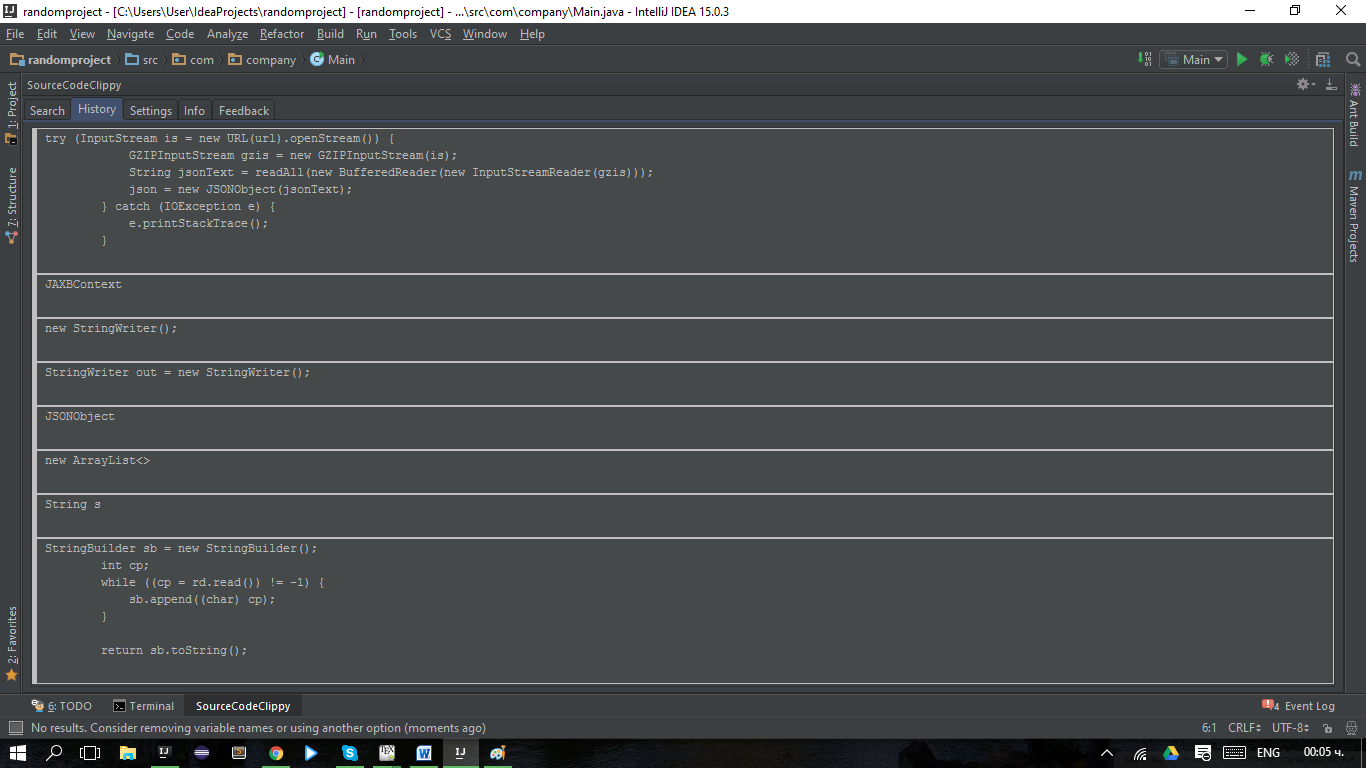
\includegraphics[scale=0.5]{tab-history}
\centering
\caption{Search history tab, Darcula IntelliJ theme}
\label{fig:history-tab}
\end{figure}

The second tab is the search history tab, which enables the user to see query searches. This feature is useful if the user wants to see previous searches in order to understand how the search 'iterations' changed the query or would like to make a search again for a past query that they cannot remember the code for - either way the user is not required to memorize or put the code searched some kind of a list they must manually update. However, if they were to decide that they would like to search with a specific query from the history, then they would need to manually copy and paste the text. The benefit is that panes are more lightweight when they do not have listeners for that task. In addition, the task of copying code was expected to occur rarely. Therefore, it was decided that query panes were kept simple for the time being.

\noindent
Each new entry is displayed at the top as a separate pane with the query text so that fresh searches are most visible. The total number of entries is 100, which can be easily made configurable. Currently, only recent query searches are shown - history is not saved to disk.


\subsection{Settings Tab}

\begin{figure}[H]
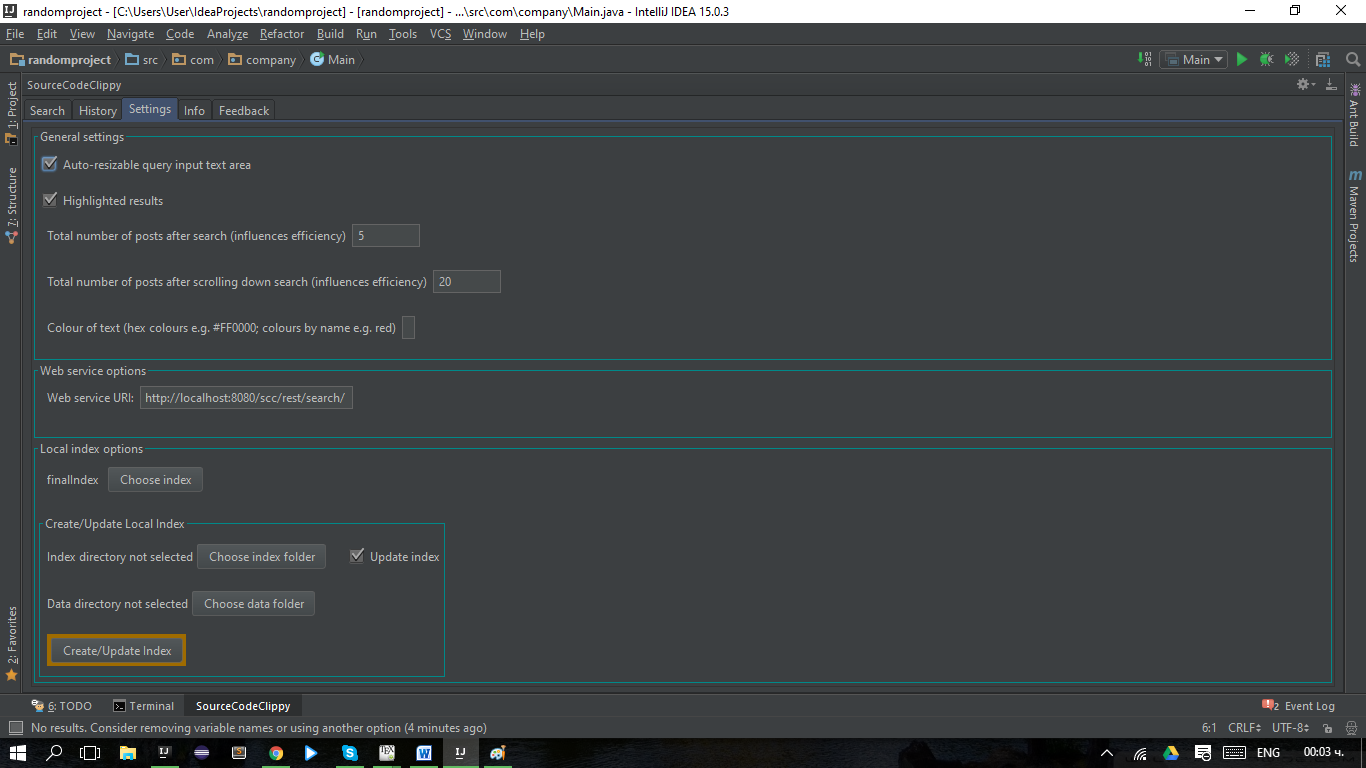
\includegraphics[scale=0.5]{tab-settings}
\centering
\caption{Settings tab, Darcula IntelliJ theme}
\label{fig:settings-tab}
\end{figure}

The third tab is the 'Settings' tab that allows configuration of the plugin. The following options are included:\\

\subsubsection{General Settings}
\begin{itemize}
\item "Auto-resizable query input text area" (check box) - offers dynamically resizable query input area or static one that is 5 rows long in terms of height and uses a scroll to show bigger input 
\item "Highlighted results" (check box) - can turn on/off highlighting of results
\item "Total number of posts" (number pane) - the number of posts after basic search using 'Enter' key. The bigger the number is, the more it will affect the efficiency of the retrieval - the user will have to wait a lot if the number is too high.
\item "Total number of posts after scrolling down search" (number pane) - controls the number of posts after extended search activated when scrolling to the bottom. The rules for efficiency mentioned for customizing the number of posts when searching apply for this setting as well.
\item "Colour of text" - The plugin provides the user with the option to change the colour of the text in posts - by typing the colour name or hex number \cite{htmlcolours}. This is done so that the plugin is not strictly dependent on the theme used by the user. In addition, it enables the them to choose to configure the look of the plugin to match their subjective preferences. Users who have some colour blindness are also predicted to  benefit from using this option.
\end{itemize}

\subsubsection{Web Service Options} 
\begin{itemize}
\item "Web service URI" (key input pane) - for setting the URI to the chosen service. The default service is set to the deployed server.
\end{itemize}

\subsubsection{Local Index Options}
\begin{itemize}
\item "Current index folder" - path to the index directory for local search
\item "Create/Update local index" - creates or updates an index by specifying index directory, data directory, and which of the two options.
\end{itemize}


\subsection{Information Tab}

\begin{figure}[H]
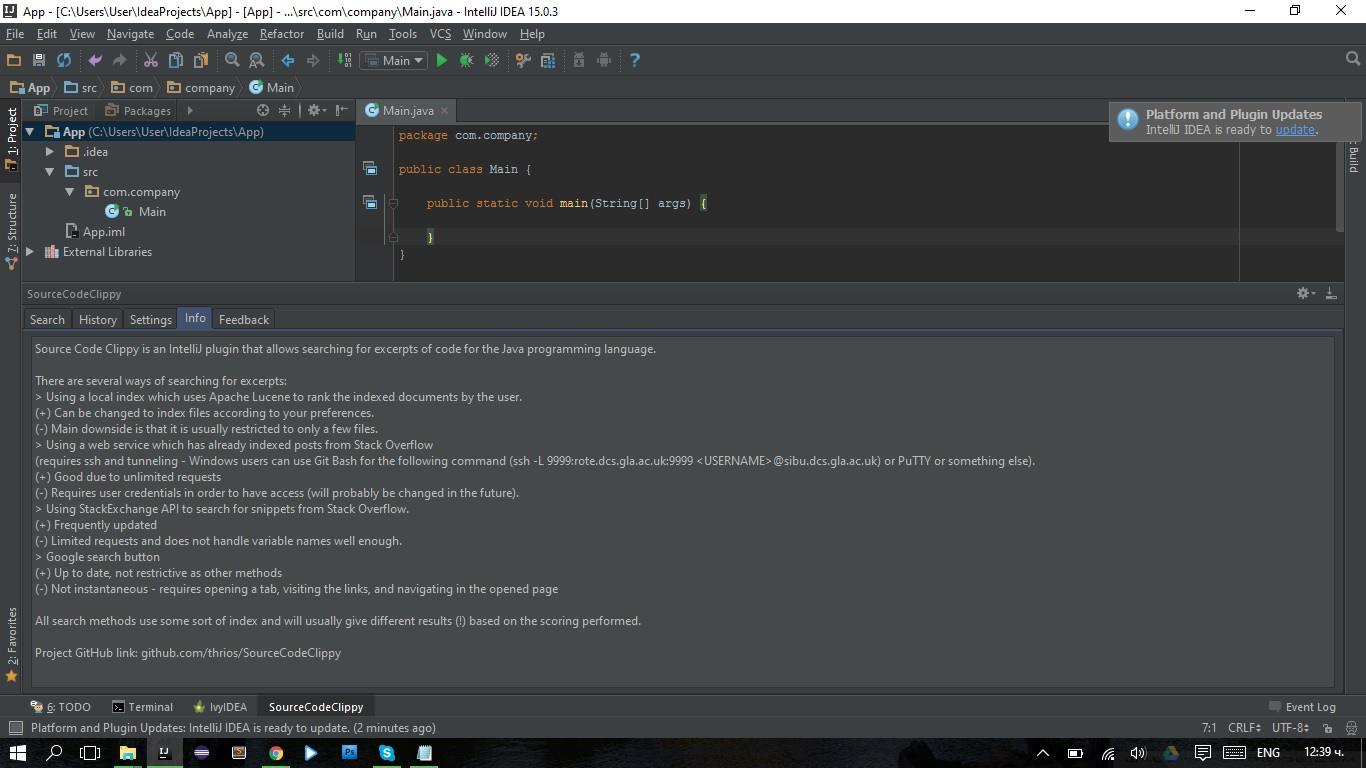
\includegraphics[scale=0.5]{tab-info}
\centering
\caption{Information tab, Darcula IntelliJ theme}
\label{fig:info-tab}
\end{figure}

The fourth tab is for plugin information which explains some details of the plugin - the purpose of the plugin, advice on which search method to use based on their advantages and disadvantages. At the bottom, the GitHub project link is added in case the user wishes to know more about the project.


\subsection{Feedback Tab}

\begin{figure}[H]
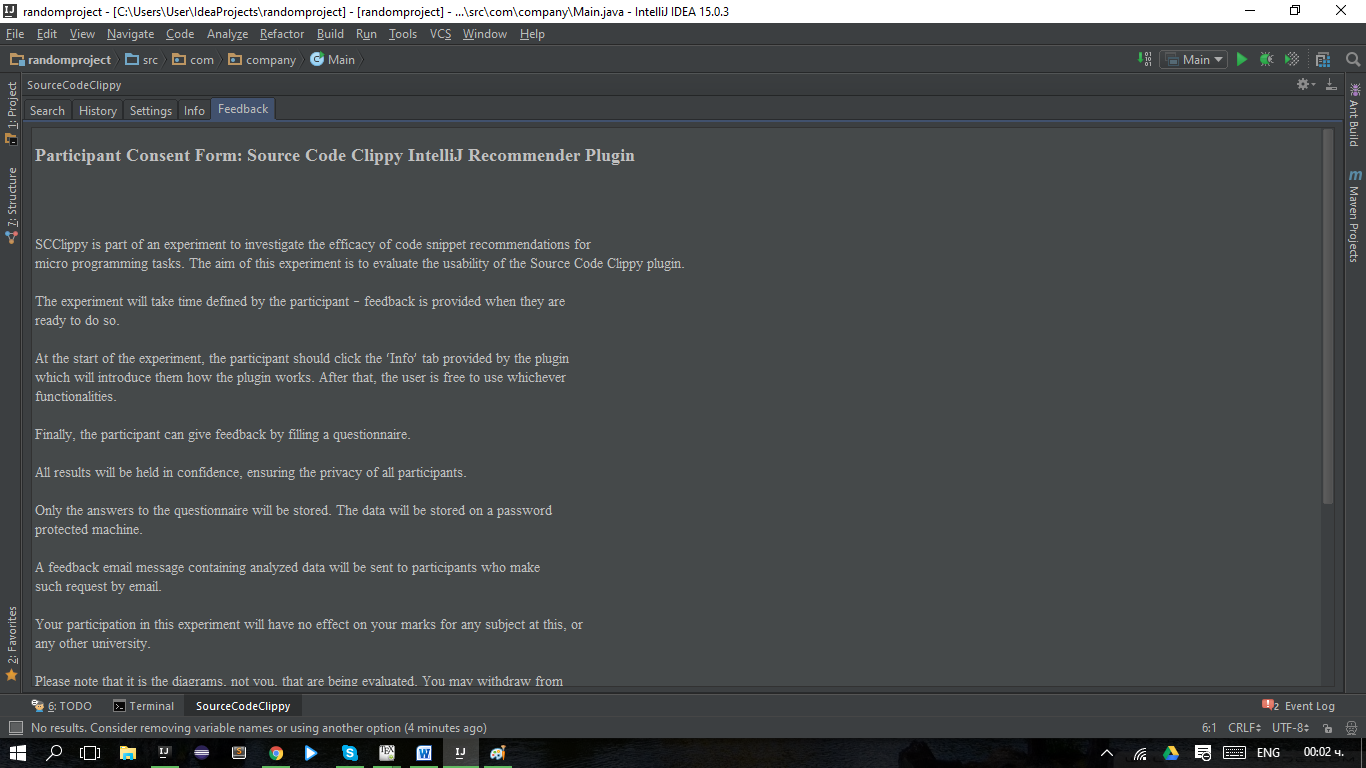
\includegraphics[scale=0.5]{tab-feedback}
\centering
\caption{Feedback tab, Darcula IntelliJ theme}
\label{fig:feedback-tab}
\end{figure}

The fifth tab contains a participant consent form and a button. The tab's components were pushed to the left (just like other tabs) make it easy for the user to have another tool opened beside Scclippy. When the button is clicked a new browser tab is opened with the online survey which the participant can fill and submit feedback by completing the required fields and even answering the optional questions. The survey was created by using an already built web application \cite{smartsurvey} ~\ref{appendix:survey}. There are benefits to this approach:
\begin{itemize}
\item Flexibility - the interface enables changes to the survey instead of creating a new one
\item Usability - it is easy to create a survey without having to code a new system
\end{itemize}




\section{Challenges}
\begin{itemize}
\item Using Terrier was initially planned for indexing and querying (http://terrier.org/), however, due to the lack of examples and information on how to use its API programmatically, the use of Lucene was considered and used instead.

\item The lack of knowledge about Information Retrieval in the early stages of the project resulted in inability to make decisions about the in-depth information retrieval platform's options at that time

\item No previous experience with developing IntelliJ plugins slowed down the process of implementation

\end{itemize}

\chapter{Evaluation}

The chapter's aim is to introduce the techniques used for evaluation of the plugin that are necessary to judge the correctness of the system and how it meets the usability and extensibility requirements.

\section{Unit Testing}
The main searching functionality of the code was tested using JUnit. The classes which have a test case are those classes responsible for searching inside the editor:

\begin{itemize}
\item StackExchangeSearch
\item WebServiceSearch
\item LocalIndexedSearch
\end{itemize}

\noindent
A major part of the code written is for the graphical user interface of the plugin. Testing that part of code is not currently supported by IntelliJ/JetBrains and therefore it was skipped. 

\section{Code Metrics}

The MetricsReloaded plugin \cite{metricsreloaded} was used to extract code metrics for the project. The code metrics gathered are for commits until the end of 22.03.2016.

\subsection{MOOD}

All code metrics from the MOOD collection \cite{mood} have been used to determine the overall quality of an object-oriented project. Below are the results for each of the criteria used. Based on those metrics, it can be seen that the results in general can be described as good - the AHF is recommended to be high; MHF, MIF/AIF depend on the system; PF is high due to many presentation logic overrides; CF should be low.

\begin{table}[H]
\small
\caption{MOOD code metrics}
\centering
\def\arraystretch{1.5}
\begin{tabular}{p{4cm}p{5cm}p{2.5cm}}
\hline
Metric & Short description & Result\\
\hline
Average hiding factor & ratio of the number of other classes a field is visible from & 0.75\\ 
Attribute Inheritance factor & ratio of what percentage of the fields for a class are due to inheritance and are not directly defined & 0.95\\
Coupling factor & the proportion of the classes coupled to other classes & 0.18\\
Method Hiding factor & the ratio of the number of classes a method is visible from & 0.35\\
Method Inheritance factor & the ratio of what percentage of the methods for a class are due to inheritance and are not directly defined & 0.04\\
Polymorphism factor & the probability that a given method will be overridden in a subclass & 3.11\\
\hline
\end{tabular}
\label{table:mood-codemetrics}
\end{table}

\subsection{Chidamber-Kemerer Metrics}

Another set of metrics for judging the quality of the code is the Chidamber-Kemerer metrics \cite{recommended-ck} \cite{recommended-ck2}. The results below show good results - response for class should not be above 50; number of children should be in the range of 0 to 10; WMC 1 to 50; DIT 2 to 5; CBO should be low; LCOM - generally good to be high, but may also mean a certain class may be doing too much.

\begin{table}[H]
\small
\caption{Chidamber-Kemerer code metrics}
\centering
\def\arraystretch{1.5}
\begin{tabular}{p{4cm}p{5cm}p{2.5cm}}
\hline
Metric & Short description & Result\\
\hline
Coupling between objects & number of classes and interface a class is coupled with & 5.28\\ 
Depth of inheritance tree & number of inheritance steps between the class and java.lang.Object & 2.64\\
Lack of Cohesion of methods & measures the cohesiveness of a class - higher values mean higher cohesion & 0.98\\
Number of children & number of direct subclasses & 0.06\\
Response for class & the number of methods in a class plus the number of methods that the class can access & 45.80\\
Weighted model complexity & cyclomatic complexity of each of the methods (in each class) & 3.11\\
\hline
\end{tabular}
\label{table:ck-codemetrics}
\end{table}

\subsection{Lines of Code}
The lines of code were counted to have statistics about the code distribution. The counting includes comments as well, but excludes white spaces.

\begin{table}[H]
\small
\caption{Package code metrics}
\centering
\def\arraystretch{1.5}
\begin{tabular}{p{3cm}p{3cm}}
\hline
Client layer & Lines of code\\
\hline
Business & 795\\
Presentation & 1368\\
\hline
Total (from above) & 2162\\
\hline
\end{tabular}
\label{table:package-codemetrics}
\end{table}

Here is an overview from a pie chart that contains the different packages and their share of code:

\begin{figure}[H]
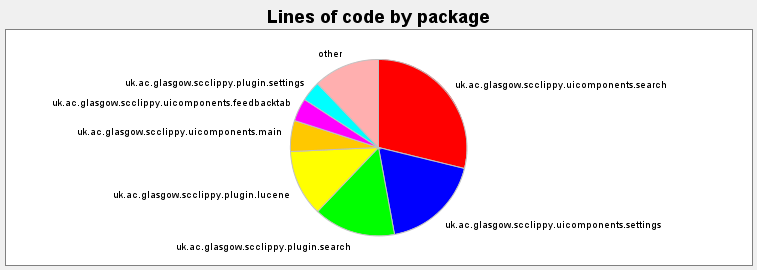
\includegraphics[scale=0.6]{code-distribution}
\centering
\caption{Code distribution for different packages}
\label{fig:code-distribution}
\end{figure}

\subsection{Language Metrics}
A table is presented to give an idea of code distribution in terms of lines and files written for each language.

\begin{table}[H]
\small
\caption{Language code metrics}
\centering
\def\arraystretch{1.5}
\begin{tabular}{p{2.5cm}p{2.5cm}p{2.5cm}}
\hline
Language & Lines of code & Files\\
\hline
Java & 2210 & 34\\
XML & 996 & 10\\
\hline
\end{tabular}
\label{table:language-codemetrics}
\end{table}

\subsection{Javadoc Coverage}
It was shown that 82.35 percent of the classes have been covered by Javadoc. The classes that have not been covered yet are straightforward implementations of features - like the info tab, the feedback tab, etc. 

\section{Acceptance Testing}

\subsection{Technique}

The evaluation with participants was decided to be carried out by giving the plugin to users who could make their own choice about whether to fill in a survey or not. The relevant documents for ethics approval were created  ~\ref{appendix:approval-part-1}, ~\ref{appendix:approval-part-2}, ~\ref{appendix:approval-part-3}, ~\ref{appendix:survey}, ~\ref{appendix:intro}, ~\ref{appendix:debrief}, ~\ref{appendix:infosheet}, ~\ref{appendix:pcf}.

\noindent
No time constraints were posed to participants since it is considered that it is best to see the results of free interaction - just like developers would naturally use the plugin in practice. This approach works best if longer period of time is given to users. However, ethics approval for conducting experiments was received more than a month after applying for it. Despite that the process of evaluation remained unchanged because there is no negative effect in the way the evaluation is done, but is rather worse in terms of the time spend to test it. Although it is generally expected that the more testing is done, the better results the results are, it is good to keep in mind that it is not known whether the old participant would test again the new functionality/improvements being added.

\subsection{Participants' Background}
The evaluation was aimed people who know Java or have started using it. The focus of finding participants was put on those who have access to the University network so that they can test searching with the Web service, which is one of the key features of the plugin. 

\subsection{User's View}
Users can participate in the evaluation of the plugin by going through the following steps:

1. Installing the plugin in IntelliJ (plugin was deployed to the JetBrains plugin repository)

2. Using the plugin's features for a desired period of time

3. Clicking on 'Feedback' tab

4. Reading the participant consent form

5. Clicking on a button, which will open the browser and take them to a survey

6. Answering at least all mandatory questions in the survey, and possibly even optional ones as well

7. Submitting the survey

\subsection{Survey Questions and Feedback}
In order to evaluate the plugin, a number of fields were asked to be filled by the participants (excluding the fields that the participant is required to agree so that he can participate). To summarize, the fields are aimed to cover the skills of the participant, the time of involvement with the plugin, the tasks performed, the satisfaction and dissatisfaction with the features and the reasons behind those two categories.

\noindent
The fields and their possible answers (if applicable) are taken directly from the survey and are listed below. The '*' symbol denotes mandatory fields which must be completed.

\subsubsection{*State your Object oriented programming skills}
\begin{itemize}
\item Beginner (4.55\%)
\item Advanced/Expert (95.45\%)
\end{itemize}

\noindent
Most of the participants (21/22) stated that they are advanced or experts when using an Object Oriented programming language. This is not surprising considering that the participants contacted were colleagues.

\subsubsection{*How long did you use the plugin for (e.g. 5 days total)?}

\begin{figure}[H]
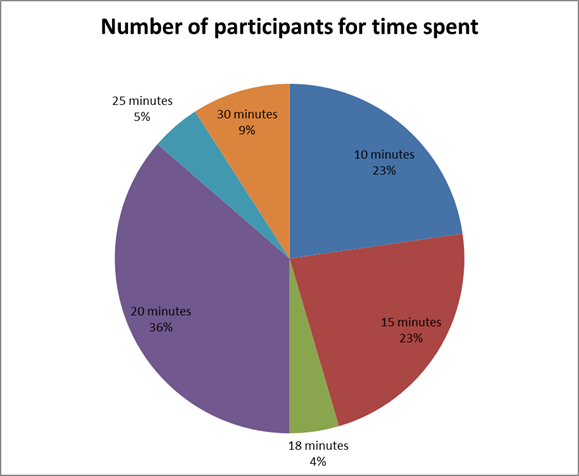
\includegraphics[scale=0.6]{participants-time}
\centering
\label{fig:participants-time}
\end{figure}

All participants used the plugin for a time range from 10 to 30 minutes (more in the next question).

\subsubsection{How often did you use the plugin (e.g. 5 minutes for 3 hours every day, 10 minutes for 1 hour 3 days a week)?}

Most participants used the plugin for day. Only one of them used it for a 2-day period. As it was mentioned, the evaluation was limited in time due to approval being received so late.

\subsubsection{What tasks did you perform?}
\begin{itemize}
\item Bug fixing (9.09\%)
\item Working on a new feature (13.64\%)
\item Prototype experiment (9.09\%)
\item Artificial task (trying out the tool) (86.36\%)
\end{itemize}

\noindent
In terms of tasks, the majority of participants (19 to be exact) aimed to try out the tool without using it for their project. Bug fixing was checked twice, another two ticks were for working on a prototype experiment, and the rest three on a new feature. From the above statistics, it is clear that some of the participants ticked more than one category. 

\subsubsection{Will you continue using the plugin?}
\begin{itemize}
\item Yes (95.45\%)
\item No (4.55\%)
\end{itemize}

It can be said that participants liked the plugin - 21 of 22 stated that they are willing to continue using it.

\subsubsection{Give an example of a task that was easier when done with the plugin (If none state ‘none’)}

The example tasks done were related to MapReduce, doing file I/O, object serialization, and other small ones like finding similar code that serves as an example for certain methods calls. Not all participants were willing to complete this field.

\subsubsection{*What do you think about the plugin in general? What do you think about the user interface and the different ways of searching for snippets?}

This is the most interesting question since it is an open question that gives the user the freedom to express themselves and share what they think about the plugin. 

\noindent
To summarize, participants liked the plugin and its features. They were happy that they could do tasks in the IDE and that it saved them time. It seems most of them used the web service search and the Stack Exchange API. There is positive feedback on that there is a button for Google search that opens the browser and searches with the query. The user interface was considered as good, a few people recommended that it should be improved (see below).

\subsubsection{What do you not like about the existing functionality of the plugin and why?}

This question is very similar to the next one (which is about thoughts about new features) by having in mind that everything disliked can be improved. Therefore, this question is focused more on what can be changed, and the next question is about what can be added.

\noindent
One of the participants mentioned that the default colour of the font is not appropriate for all IntelliJ themes. This issue needs investigation to see whether IntelliJ provides options to detect the colour theme used, and in case it does not, a setup window can appear the first time the plugin is loaded to allow the user to customize the colour. 

\noindent
There was a complaint about the interface - it was suggested that there should be a button beside the query pane to make the search request since it is not obvious to everyone that pressing 'Enter' is faster and provides the same functionality. This can easily be implemented.

\noindent
The arrow at the bottom of each snipper gives the impression it is clickable. The participant thought that details would appear for the particular post. There is a simple solution to this problem - the arrow can be replaced by something else.

\noindent
A participant also mentioned that the search bar should always be at the top so that they can easily modify the search query without the need to scroll up so that the plugin is more usable. Implementation wise, this can be done without much effort - by having the scroll applied for the panel responsible for the posts instead of having that scroll the whole tab as it currently is.

\noindent
Consecutive searches with the same query appear in history. This can be fixed making a check that will compare the last entry and the new one. Furthermore, a counter can be added to serve as an indication how many times a query is searched - perhaps the user switched the method of searching and

\noindent
The 'Info tab' can contain more information about the plugin's features such as what can be double clicked and perhaps a more detailed description on how to search with an example.

\subsubsection{Do you think there are any additional features that need to be implemented?}

A participant recommended that there should be an option that allows automated removal of variable names since they are less meaningful than other code and are and the StackExchange API returns only results that match all terms in the query.

\noindent
The history tab can have filters or text search in order to make the process of finding the desired query faster.
Include more information in the 'info tab' - for example, double clicking inserts a code snippet in the editor.

\noindent
One of the proposals is to have support for languages other than Java. It is not something new - the improvement has been intended to be included in the plugin in the future.

\noindent
Have a shortcut for searching with the query and maybe have other shortcuts as well

\noindent
A nice feature suggested was allowing the user to mark all the results that the user has read as 'Read' or maybe even the plugin can automatically track the posts seen that the user has spend time on.

\noindent
Some users were interested in the comments for a particular post so that they do not have to open the browser. This can be implemented by using the Stack Exchange API.

\noindent
A participant has the idea to have automatic update on the query when a text in the post is selected - the plugin only does this for text in the editor. On the one hand, this is good because the user does not need to copy-paste the piece of code, however, on the other, this can delete the current search query. Nevertheless, it is possible to have this feature - by either providing a check box to enable/disable this functionality; by having a button that will allow the user to go back to the previous queries; or by making the automatic copy-paste to require a right click after selection where the option to paste the query will appear - the user would not need to move his mouse and paste the text.

\noindent
One of the comments included how good code snippet insertion with web search is. The user wishes to be able to do the same for other types of search such as Stack Exchange API. Currently, the plugin uses special tags for the web service that indicate that a piece of code is there. In order to implement the new feature, the user should indicate where the snippet starts and ends. The best way to do that is to track mouse selection. However, a further action is needed by the user (maybe right clicking and then click on 'import into editor') so that text is not automatically included each time the user decides to use their mouse to select a given piece of text. 

\noindent
Finally, a participants would like a new setting that will allow them to change to the size of the text for every post. It is possible to include this feature by modifying the CSS of each post just like highlighting is done currently.

\subsection{Feedback Summary}
From the participants opinions, it can be fisrtly be concluded that there is a list of changes that need to be done in order to improve the usability of the system even more than it currently is. The good side is that most of the corrections needed are not expected to take much time, especially when considering that solutions to the respective problems were described. Secondly, the all suggested improvements are about extending the functionality of the plugin. It must be said that all the changes proposed by the users seem possible to implement and are envisioned that the system will likely benefit from their implementation. It is important to note that only if these additions are done correctly as described will they become effective.   

\chapter{Conclusion}

\section{Project Outcome}

Source Code Clippy is a configurable plugin that enables the search of excerpts from different sources, along with other helpful functionality. 

\noindent
The plugin was successfully implemented, tested, deployed (to the JetBrains repository) and evaluated. All requirements were fulfilled, except one 'would-have' responsible for making search more sophisticated - adding tags and/or assigning less weight to variable names as they typically tend to be more irrelevant for a given query.

\noindent
The evaluation showed that the plugin is liked by the participants. Like any other system, there are still improvements to be made, some of which were suggested from the feedback gathered.

\section{Future Work}

\subsection{Using the Cloud}
In the future, a cloud solution can be used for the web service so that it is accessible by everyone, while also being highly available. 

\subsection{Intelligent Search}
It is reasonable to say that the plugin could benefit from having a more intelligent search which can be done using various techniques:

- More weight could be assigned to keywords and relevant code so that less important code such as variable names are not regarded as significant. 

- Making use of tags could prove to be beneficial by matching the user's needs - specifically when they would like to get results only from a subset of the data. Tags can be included for all three types of search (local index, web service, Stack Exchange API).

- Extracting other information from the provided database could help to include more data when returning results or for filtering purposes. For example, one or more of the following columns could be taken into account: 'creationdate', 'viewcount', 'answercount', 'commentcount', 'favouritecount'. The Stack Exchange API \cite{stackexchange} can also be used more frequently e.g. to retrieve comments for posts; excerpts can be allowed to be customized more by the user.

\subsection{Other Possible Extensions}
The plugin can be extended to have:

\begin{itemize}
\item All the improvements gathered through evaluation that were mentioned
\item Support for multiple languages
\item Caching of results (not much beneficial since retrieval is fast)
\item Storing functionality to save search history permanently
\item Options for better interaction with Stack Exchange - login/logout, notification when someone has answered the user's question
\end{itemize}

\section{Learning Outcomes}

At the beginning of this project, there was a lack of experience on how to build an IntelliJ plugin and insufficient knowledge about information retrieval along with its according available platforms. However, by going through the process of creating the plugin, the required skills were learned. In addition, the existing skills of developing software were enhanced by making decisions about ideas and their implementation in practice.

%%%%%%%%%%%%%%%%%%%%
%   BIBLIOGRAPHY   %
%%%%%%%%%%%%%%%%%%%%
\bibliographystyle{ieeetr}
\bibliography{bibliography}

%%%%%%%%%%%%%%%%
%              %
%  APPENDICES  %
%              %
%%%%%%%%%%%%%%%%

\begin{appendices}
\chapter{Appendix}

\section{Ethics Approval Form}

\begin{figure}[H]
\centering
\fbox{
\includegraphics[scale=0.5]{appendices/approval-part-1.pdf}}
\caption{Ethics approval form - page 1}
\label{appendix:approval-part-1}
\end{figure}

\begin{figure}[H]
\centering
\fbox{
\includegraphics[scale=0.5]{appendices/approval-part-2.pdf}}
\caption{Ethics approval form - page 2}
\label{appendix:approval-part-2}
\end{figure}

\begin{figure}[H]
\centering
\fbox{
\includegraphics[scale=0.5]{appendices/approval-part-3.pdf}}
\caption{Ethics approval form - page 3}
\label{appendix:approval-part-3}
\end{figure}

\section{Survey}
\begin{figure}[H]
\centering
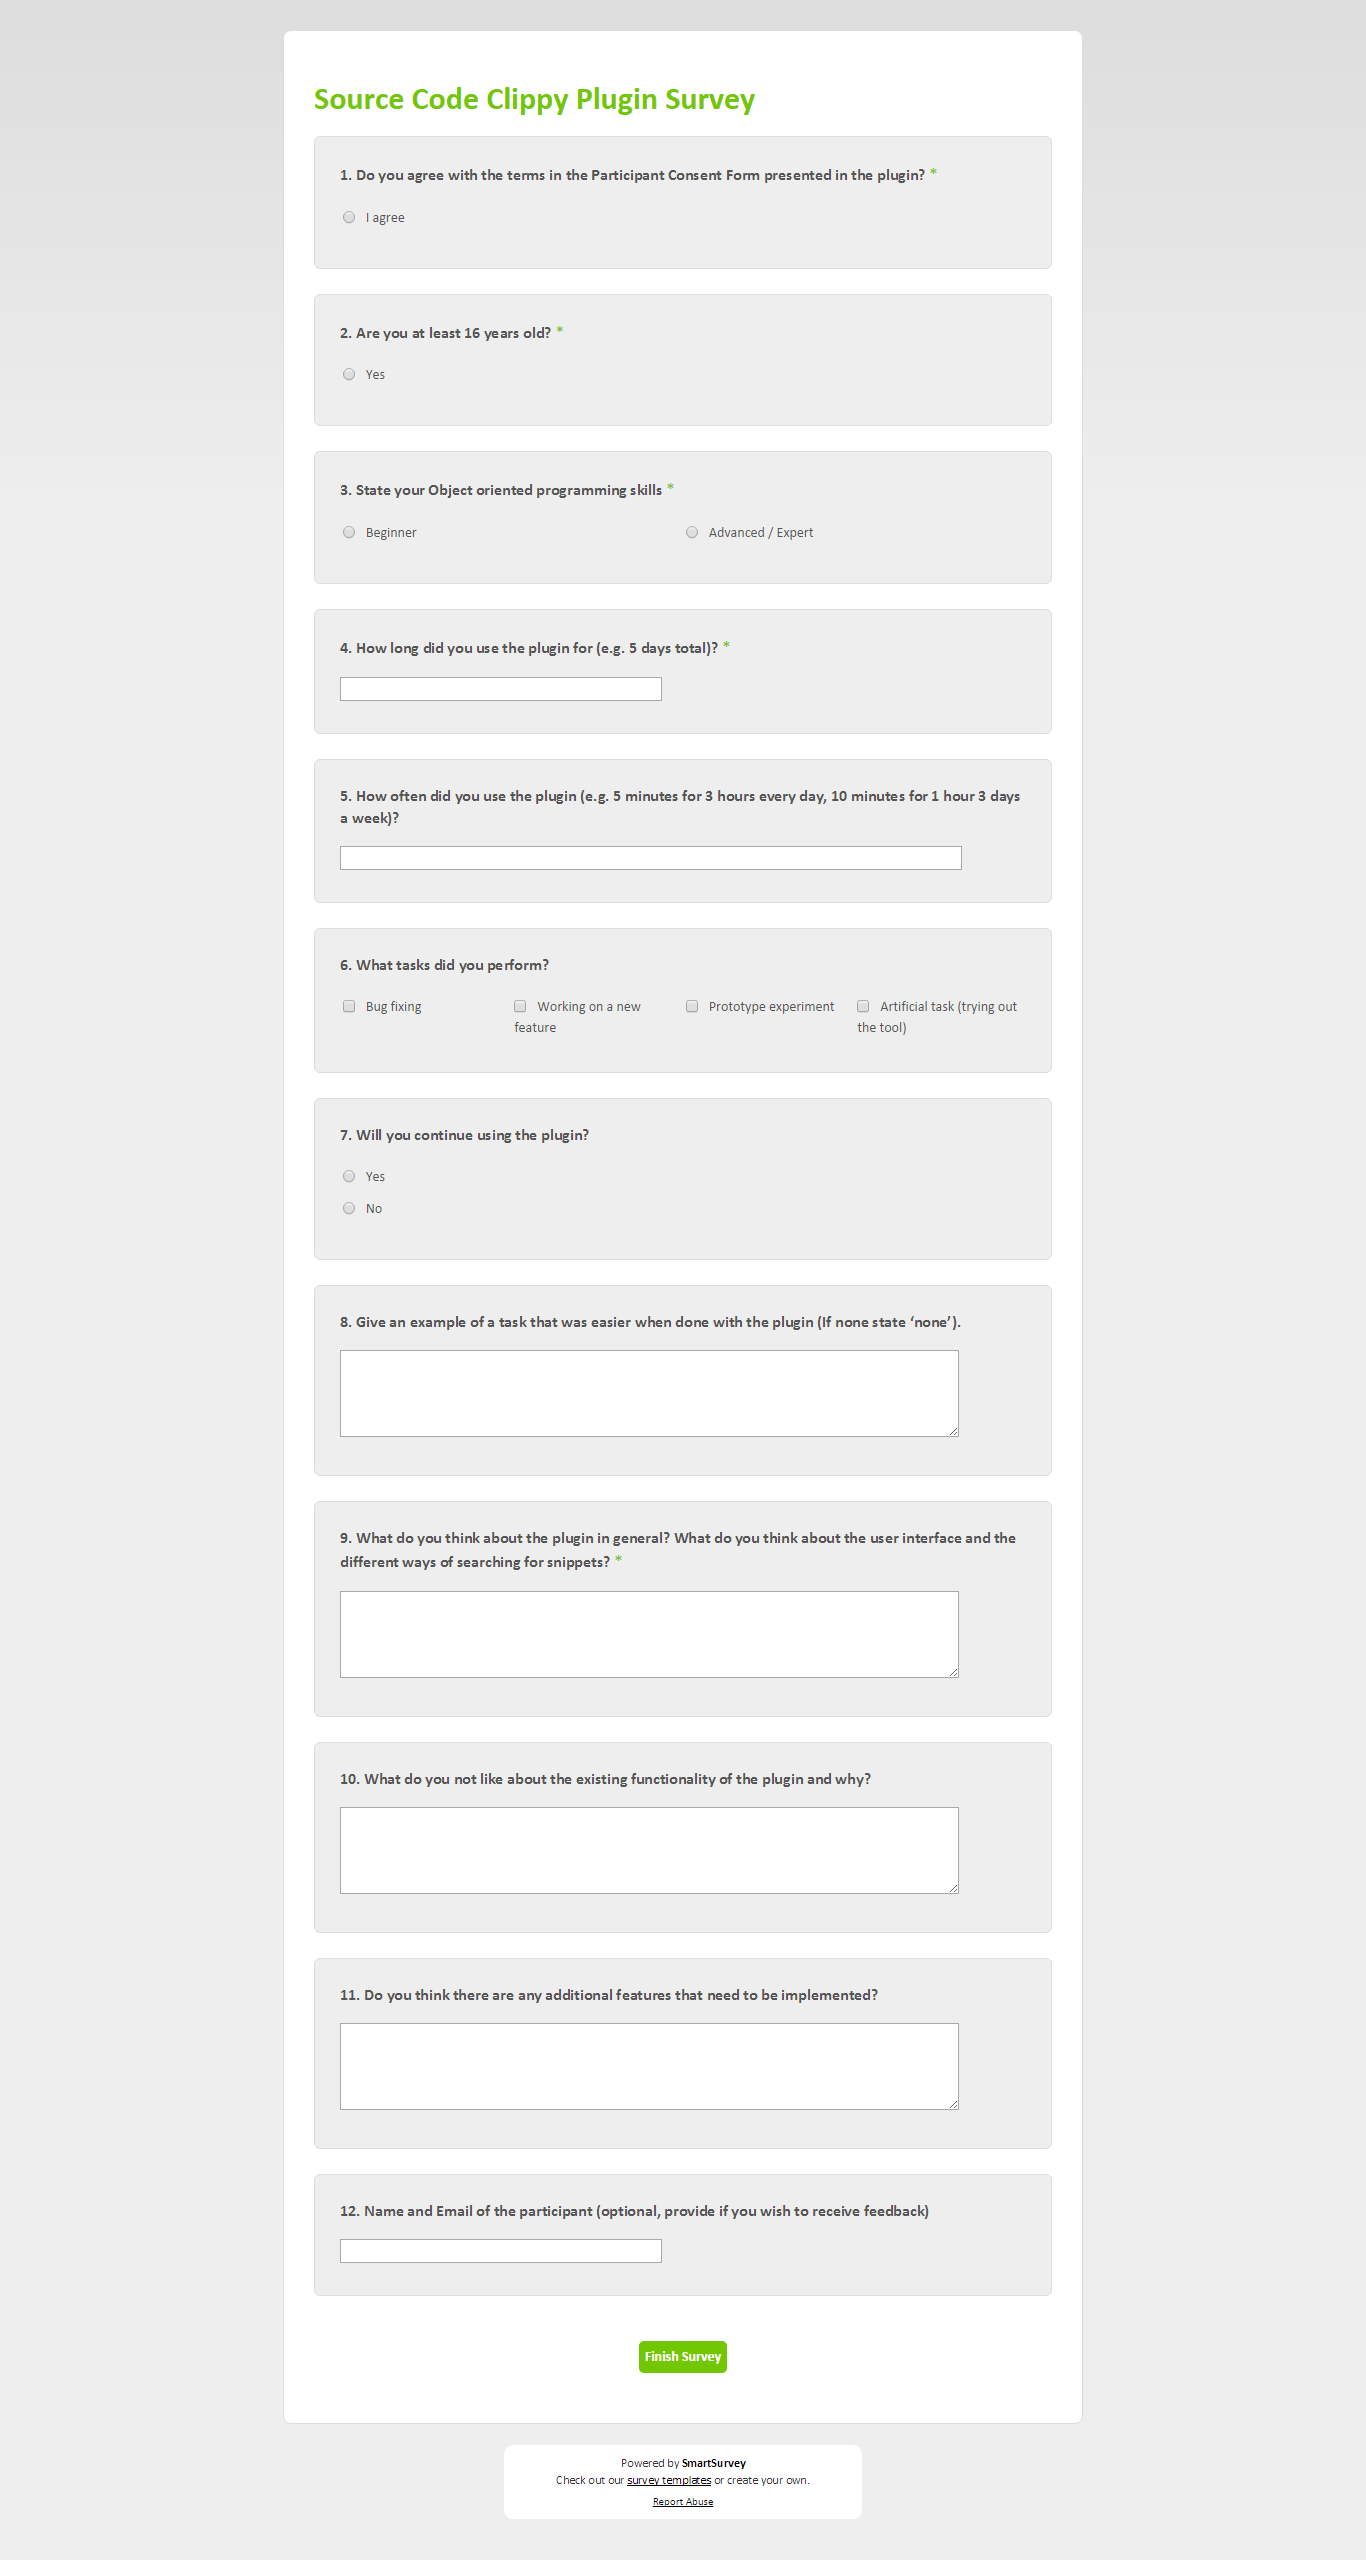
\includegraphics[scale=0.25]{appendices/survey.png}
\caption{Survey}
\label{appendix:survey}
\end{figure}

\section{Introduction script}
\begin{figure}[H]
\centering
\fbox{
\includegraphics[scale=0.75]{appendices/scc-introduction.pdf}}
\caption{Introduction script}
\label{appendix:intro}
\end{figure}

\section{Debrief script}
\begin{figure}[H]
\centering
\fbox{
\includegraphics[scale=0.75]{appendices/scc-debrief.pdf}}
\caption{Debrief script}
\label{appendix:debrief}
\end{figure}

\section{Information Sheet}
\begin{figure}[H]
\centering
\fbox{
\includegraphics[scale=0.75]{appendices/scc-infosheet.pdf}}
\caption{Information Sheet}
\label{appendix:infosheet}
\end{figure}

\section{Participant consent form}
\begin{figure}[H]
\centering
\fbox{
\includegraphics[scale=0.75]{appendices/scc-pcf.pdf}}
\caption{Participant Consent Form}
\label{appendix:pcf}
\end{figure}

\end{appendices}

\end{document}
